%pdflatex main.tex
\documentclass[12pt]{article}
\usepackage{natbib}
\usepackage[francais]{babel}
\usepackage{natbib}
\usepackage{url}
\usepackage[T1]{fontenc}
\usepackage[utf8x]{inputenc}
\usepackage{amsmath}
\usepackage{graphicx}
\usepackage[table,xcdraw]{xcolor}
\usepackage{wrapfig}
\usepackage{float}
\usepackage[rightcaption]{sidecap}
\graphicspath{{images/}}
\usepackage{titlesec}
\setcounter{secnumdepth}{4}

\titleformat{\paragraph}
{\normalfont\normalsize\bfseries}{\theparagraph}{1em}{}
\titlespacing*{\paragraph}
{0pt}{3.25ex plus 1ex minus .2ex}{1.5ex plus .2ex}
\usepackage{amsthm}
\usepackage{parskip}
\usepackage{fancyhdr}
\AddThinSpaceBeforeFootnotes
\FrenchFootnotes
\usepackage{xfrac}
\usepackage{esvect}
\usepackage{vmargin}

\usepackage{datetime}
\newdate{date}{23}{06}{2016}
\date{\displaydate{date}}

\usepackage{gensymb}
\setmarginsrb{3 cm}{2.5 cm}{3 cm}{2.5 cm}{1 cm}{1.5 cm}{1 cm}{1.5 cm}

\title{Big Data}								% Title
\date{\today}											% Date

\makeatletter
\let\thetitle\@title
\let\theauthor\@author
\let\thedate\@date
\makeatother

\pagestyle{fancy}
\fancyhf{}
\rhead{\theauthor}
\lhead{\thetitle}
\cfoot{\thepage}
\newtheorem*{rappel}{Rappel}
\newtheorem*{nota}{N.B}
\newtheorem*{req}{Remarque}
\begin{document}

%%%%%%%%%%%%%%%%%%%%%%%%%%%%%%%%%%%%%%%%%%%%%%%%%%%%%%%%%%%%%%%%%%%%%%%%%%%%%%%%%%%%%%%%%

\begin{titlepage}
	\centering
    \vspace*{0.5 cm}
    
\includegraphics[scale = 0.75 ]{logo1}\\[1.0 cm]	% University Logo
    \textsc{\LARGE EISTI}\\[2.0 cm]			% University Name
    \rule{\linewidth}{0.2 mm} \\[0.5 cm]
    { \huge \bfseries \thetitle}\\
    \rule{\linewidth}{0.2 mm} \\[1.5 cm]
	\textsc{\Large Généralités sur le Big Data}\\[0.5 cm]	% Course Code
	
	
	\begin{minipage}{0.4\textwidth}
	\centering
		\begin{center} \large
		Maxime LUNDQUIST \\
		Mandry MBUNDU \\
		David RIGAUX \\
		Mehdi DALAA \\
		\textsc{\large CPI1 C2}\\[0.5 cm]		% Course Name
			\end{center}
			\end{minipage}~
			\begin{minipage}{0.4\textwidth}
	\end{minipage}\\[0.8 cm]
	{\large \displaydate{date}}\\[1 cm]
	\vfill
	
\end{titlepage}

%%%%%%%%%%%%%%%%%%%%%%%%%%%%%%%%%%%%%%%%%%%%%%%%%%%%%%%%%%%%%%%%%%%%%%%%%%%%%%%%%%%%%%%%%

\tableofcontents
\addtocontents{toc}{~\hfill\textbf{Page}\par}
\pagebreak

%%%%%%%%%%%%%%%%%%%%%%%%%%%%%%%%%%%%%%%%%%%%%%%%%%%%%%%%%%%%%%%%%%%%%%%%%%%%%%%%%%%%%%%%%
\section{Introduction}
Aujourd'hui, en 24h nous générons environ 2,5 trillions \footnote{1 Trillion $= 10^{18}$ } d'octets de données. Au point qu'en l'espace de deux ans nous avons créé 90\% des données présentes dans le monde. Ces données en question sont de tout type et proviennent de partout : les messages que nous nous envoyons, les photos et vidéos que nous publions, les capteurs métrologiques, les enregistrements transactionnels d'achats en ligne, les signaux GPS et bien d'autres encore. Ces données sont appelées Big Data ou encore volumes massifs de données. Le Big Data désigne un ensemble très volumineux de données qu'aucun outil classique de gestion de bases données ou de gestion de l'information ne peut vraiment travailler. Avec un marché potentiel de plus de 50 milliards de dollars dans les 10 prochaines années \emph{(selon une étude Gartner)}, il est sûr que le Big Data va jouer, dans les prochaines années, un rôle encore plus déterminant qu'aujourd'hui dans la manière dont le monde numérique va évoluer et la manière dont les entreprises et gouvernements vont revoir leur mode de gestion de l'information. La complexité de ce nouveau concept et l’impact de ce dernier sont tels qu’il est important de saisir dès maintenant les caractéristiques du Big Data. \par
\emph{Mais qu'est-ce vraiment le Big Data ?} Malheureusement, aucune définition précise ou universelle ne peut être donnée au Big Data dû au fait qu'il s'agit d'un objet complexe polymorphe, sa définition varie alors selon les communautés qui s'y intéressent en tant qu'usager ou fournisseur de services.\\ Le Big Data est un système technique dual en apportant des bénéfices mais peut tout de même générer des inconvénients. Les inventeurs du Big Data, qui sont les géants du web\footnote{Google, Yahoo, Facebook, etc.}, le présente comme une solution dessinée pour permettre à tout le monde d’y accéder en temps réel  des bases de données géantes. D'après \emph{Gartner} \footnote{Gartner, inc. est le leader mondial dans les recherches informatiques et conseils.}, on peut le définir comme outil répondant à une tripe problématique, appelée : \textbf{règle des 3V}. Le premier V représente le \textbf{Volume} de données considérable à traiter. Puis, le deuxième V décrit  une grande \textbf{Variété} d'informations qui viennent de diverses sources, non structurées, organisées, open et pleins d'autres. Et finalement, le troisième et dernier V incarne le niveau de \textbf{Vélocité} à atteindre, c'est-à-dire atteindre une certaine fréquence de création, de collecte et de partage de ces données. 
\begin{figure}[H]
\centering
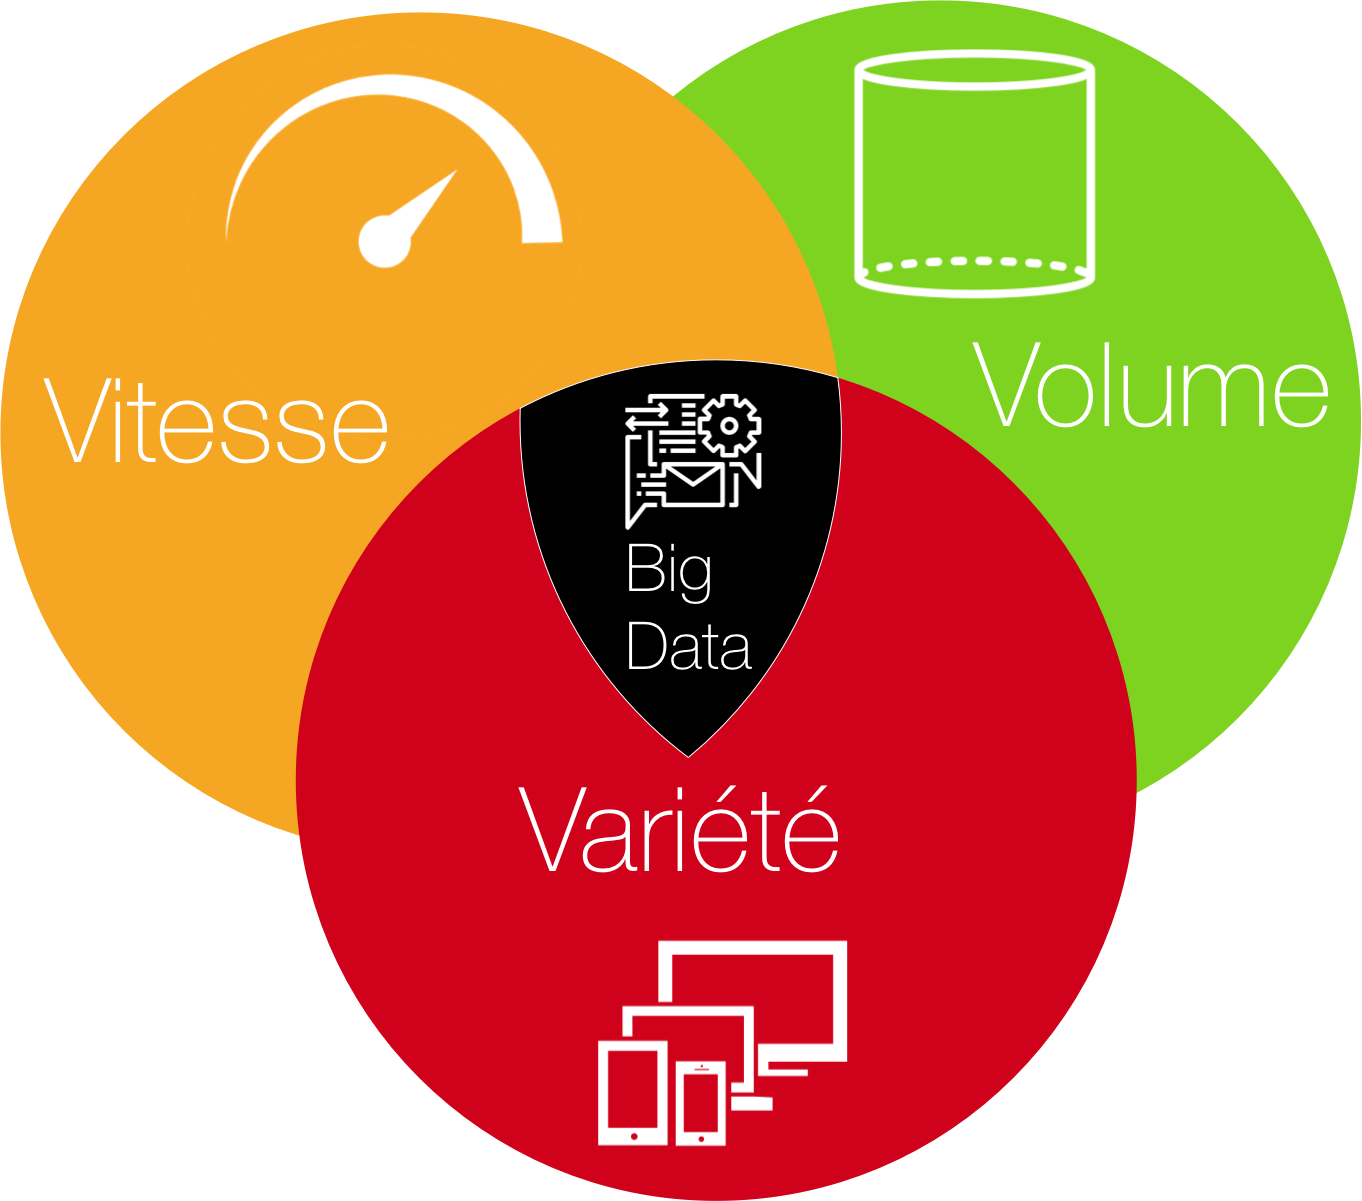
\includegraphics[width=0.45\textwidth]{3V}
\caption{Les 3V du Big Data}
\end{figure}
Cependant, au cours du temps ces qualificatifs ont évolué, avec une vision davantage économique portée par le 4ème V de la définition, celui de \emph{Valeur}, et une notion qualitative véhiculée par le 5ème V, celui de la Véracité des données, c'est-à-dire de disposer de données fiables pour le traitement. 
\begin{figure}[H]
\centering
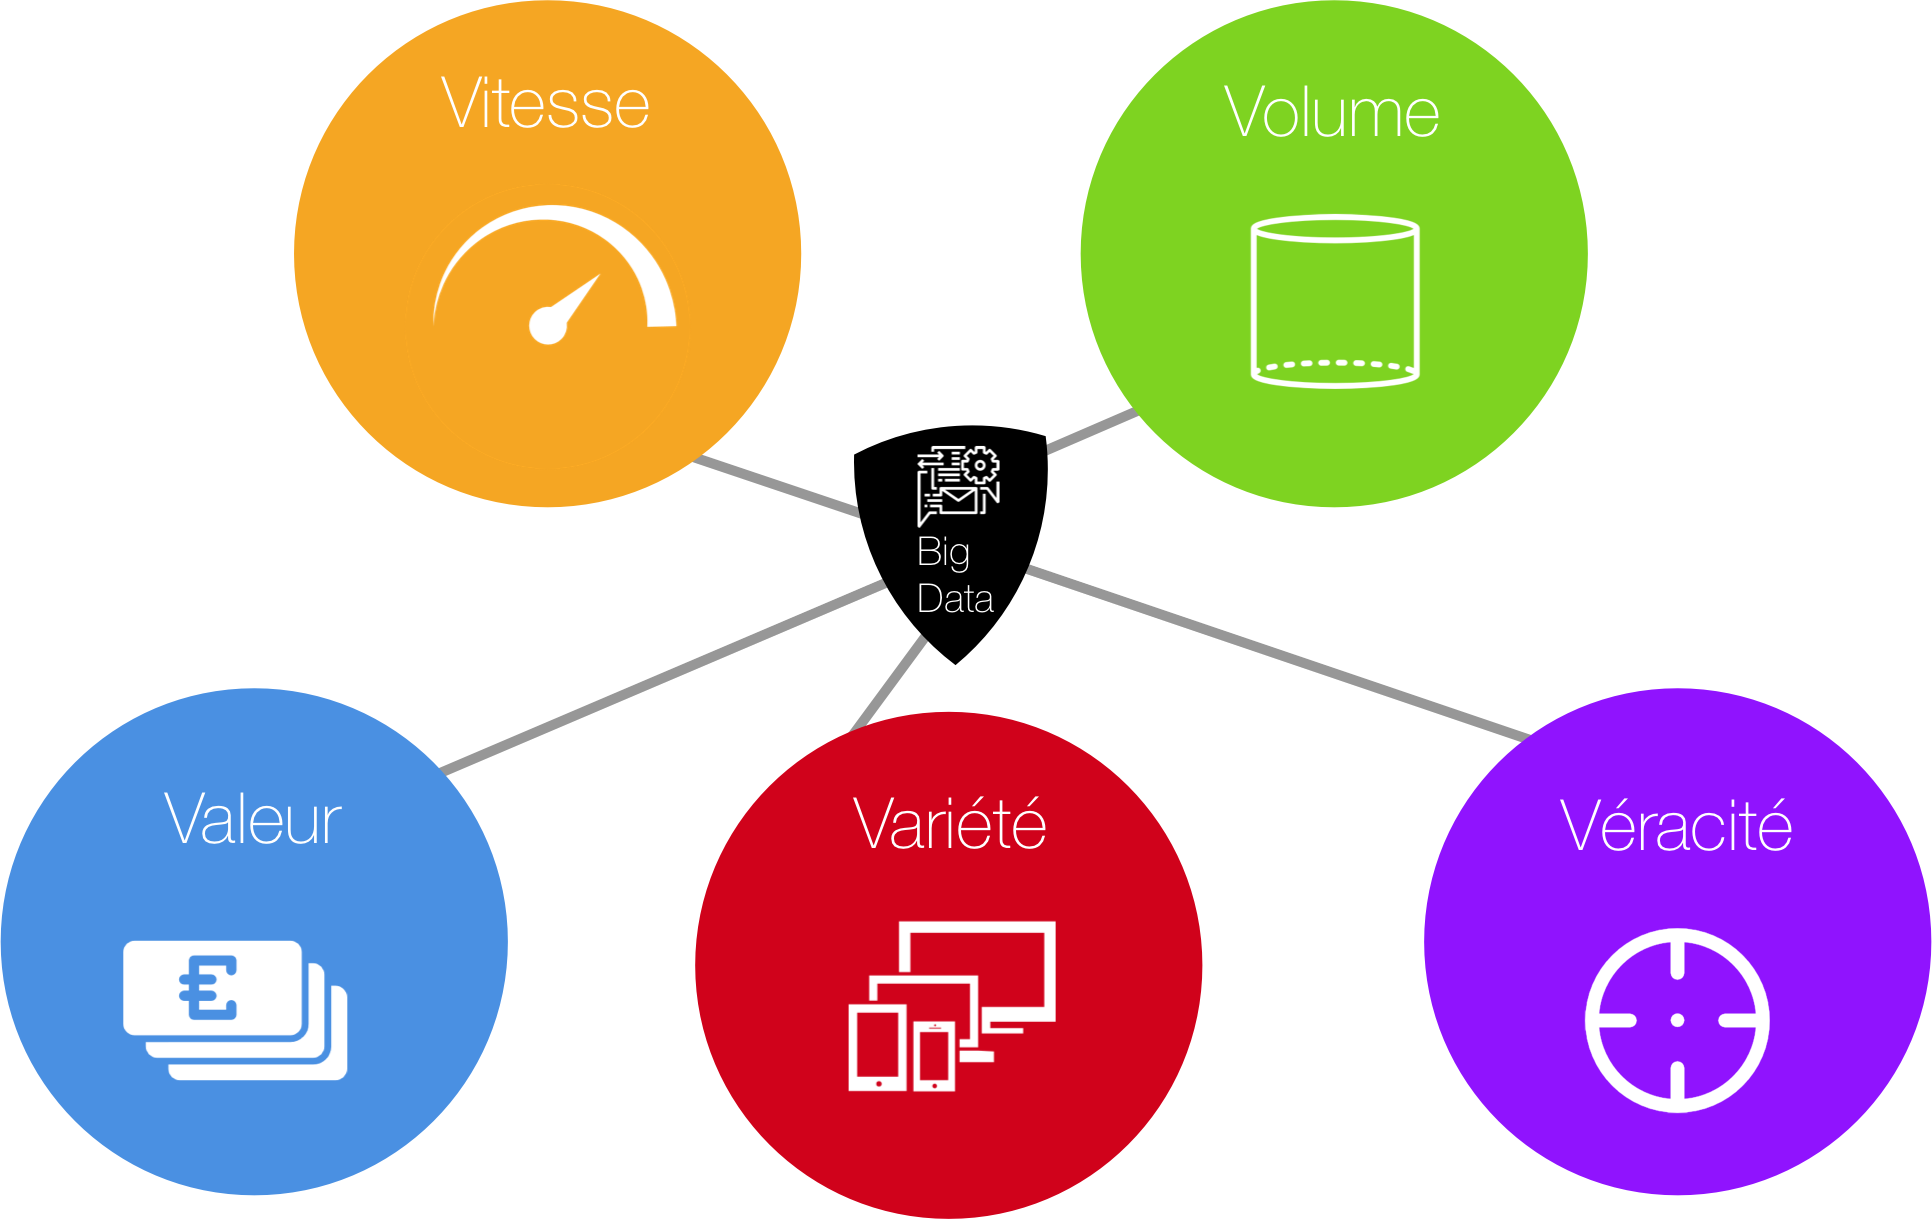
\includegraphics[width=0.75\textwidth]{5V}
\caption{Les 5V du Big Data}
\end{figure}
\section{Historiquement, comment en est-on arrivé au Big Data ?}
Le Big Data défini donc des données trop volumineuses pour être manipulé à l’aide de bases de données relationnelles. C’est-à-dire une base de données où l'information est organisée dans des tableaux à deux dimensions. L’arrivée du Big Data a donc contribué à un changement dans la gestion des données et dans l’utilisation des systèmes servant à les manipuler.\par
Le besoin d’organiser les données, potentiellement de grandes quantités, afin d’en optimiser la conservation et la restitution, a toujours été au cœur de l’informatique. Ce besoin s’est d’autant plus fait ressentir entre 1965 et 1975 avec le développement de l’informatique dans les grandes entreprises. C’est donc en 1970 que l’informaticien britannique d’IBM  Edgar F. Codd définit le modèle de données relationnel qui a pour avantage de séparer la gestion physique et la gestion logique des données. Les systèmes de gestion de base de données relationnels deviennent alors très rapidement les systèmes dominants dans la gestion de base de données et sont exploités avec le langage informatique SQL créé en 1974.

\par
Avec le développement des technologies mobiles, les échanges d’informations numériques se sont grandement multipliés. Ainsi le début du XXIe siècle est marqué par une explosion considérable du volume de donnée manipulé à travers la planète. En effet, que ce soit les données scientifiques, les données liées aux réseaux sociaux, les bases de données médicales, ou encore les indicateurs économiques et sociaux, tous les types de données ont vu leur volume croître considérablement. Ce volume énorme qui se compte aujourd’hui en pétaoctets (100 000 téraoctets), manipulé de part et d’autre du globe est représentatif du Big Data. 
\begin{figure}[H]
\centering
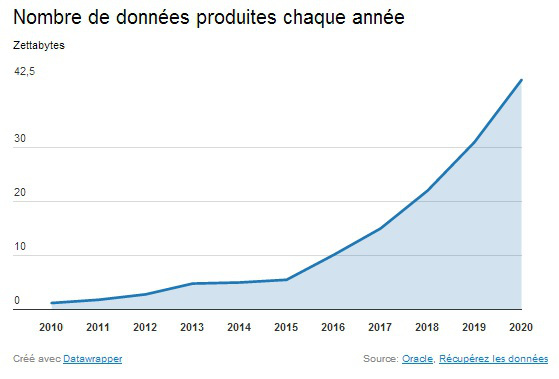
\includegraphics[width=0.75\textwidth]{graphe}
\caption{Graphique représentant le nombre de données produites chaque année}
\end{figure}
En revanche, on ne peut pas dire que l’on est dans une situation de type Big Data à partir de telle ou telle volumétrie. Le Big Data varie d’un secteur à un autre, car les outils et les volumes de données gérées ne sont pas identiques. Le Big Data varie également d’une décennie à l’autre, car le volume de données est en expansion continue. 
\par
La gestion et le traitement de ces volumes de données sont considérés comme un nouveau défi de l’informatique. Pour cause, les systèmes de gestion de base de données relationnels sont incapables de gérer de telle masse de données. D’où la naissance d’une famille de système de base de données nommé NoSQL.
\par
Les grandes sociétés du web sont les organismes les plus concernés par la manipulation de grands volumes de données. C’est pourquoi elles ont été les premières confrontées aux limites des systèmes de gestion des bases de données relationnelles. Afin de répondre à ces limites ces entreprises ont commencé à développer leurs propres systèmes de gestion de bases de données NoSQL pouvant fonctionner sur des architectures matérielles distribuées et permettant de traiter des volumes de données importants. 
Voici quelques exemples d’entreprises et de leur système de gestion de bases de données NoSQL :
\begin{itemize}
\item Google avec GFS puis Big Table 
\item Amazon avec Dynamo
\item Facebook avec Cassandra Project puis Hbase
\item Baidu avec Hypertable
\end{itemize}
\par
Les grandes entreprises du web sont donc les pionniers du modèle NoSQL.
\par
Réalisant le potentiel de cette technologie, l’américain Doug Cutting s’inspira de GFS et Big Table pour lancer le prototype open source Hadoop qui grâce à son modèle de programmation et à son système de fichier hautement distribué est capable de gérer de gigantesques quantités de données non structurées. Hadoop est une technologie qui fait aujourd’hui référence dans l’univers du Big Data.
\par
Les performances des systèmes de gestion de base de données NoSQL sont restées bonnes malgré la forte augmentation de la demande. Il a un simplement fallut multiplier le nombre de serveurs, ce qui fut une solution raisonnable  avec la baisse des coûts de ces derniers.
\par
Le modèle relationnel ne s’est pas effacé pour autant. Il reste même majoritaire dans le traitement de données et est largement répandu dans les entreprises. Utilisé pour une quantité d'informations et un nombre d'utilisateurs typiques d'une entreprise. Il montre cependant ses limites lorsqu'il est utilisé dans un périmètre plus large, tel qu'un site web populaire, fréquenté par des millions de visiteurs dans le monde entier. Les systèmes de gestion de base de données relationnels exigeraient alors des logiciels et des ordinateurs coûteux ainsi que des compétences en optimisation peu répandues. Ce segment de marché est de ce fait occupé par les logiciels NoSQL, conçus spécifiquement pour un usage de type Internet.
\pagebreak
\section{Domaines d'applications}
Avant l'émergence du Big Data, des cas d'usages de cette technologie existaient déjà.
Cependant, grâce à ce dernier, nous pouvons aller beaucoup plus vite et traiter une quantité beaucoup plus importante de données.Les grandes utilisations du Big Data sont : 
\begin{itemize}
\item pressentir la naissance d’une tendance,
\item prédire l’évolution d’un phénomène,
\item repérer des corrélations pour optimiser une stratégie,
\item faire des contrôles pour découvrir une fraude,
\item organiser une communication virale,
\end{itemize}
On voit par ces cas d'usages que le Big Data touche tous les secteurs et toutes les sociétés (néanmoins une très grande partie) et nous allons vous présenter  l'impact du big data dans le marketing et la surveillance.
\subsection{Le Marketing}
Lorsque l'on pense, Big Data, on pense naturellement dans un premier temps au marketing. 
Par le biais des cartes de fidélité, une grande surface par exemple peut visualiser les achats d'un client et par le biais du big data, donc du traitement de ces données effectuer une analyse prédictive et ainsi pouvoir changer le positionnement de ces produits par exemple afin de mieux les organiser selon les désirs des clients. \par
Mais le big data dans l'amélioration du marketing ne se limite pas à cela, il y a ce que l'on appelle la " e-réputation ", c'est-à-dire son image sur les réseaux sociaux. Si une enseigne lance un nouveau produit, il va être très important pour elle de voir ce qu'en disent les internautes sur la toile, les entreprises voient alors les réseaux sociaux comme le reflet de l'opinion publique. \par
 Le Big Data permet alors de visualiser en direct l'impact de sa marque, comment elle est perçue par le public afin de pouvoir anticiper les mauvaises critiques, les fausses rumeurs qui pourraient ruiner l'image de l'enseigne, faire chuter son cours en bourse ou encore fortement atteindre les ventes d'un produit en permettant à l'équipe chargée de la communication d'intervenir en direct. Le Big Data permet donc de faire d'importantes économies.\par
En étudiant les habitudes de ses consommateurs par l'exploitation des données obtenues par les méthodes citées juste avant, une entreprise peut alors lancer une fidélisation de ses clients qui est le pilier du marketing viral.\par
C'est le cas de Globe Telecom, opérateur de Télécom, a monté un projet basé sur des technologies Big Data qui permet la détection de l’épuisement du crédit des cartes téléphoniques prépayées en fonction des modes de consommation (durée et fréquence des appels, nombre de SMS par jour). L’opérateur était intéressé par ce type d’analyse, car sa clientèle est très volatile. Ce procédé leur a permis de réduire de 95\% les coûts des opérations marketing et d’améliorer de 600\% la pertinence de leurs offres promotionnelles tout en fidélisant une plus grande partie des clients.\par
L'analyse du comportement est également un point clé du big data, nous avons au départ parlé des cartes de fidélité, mais l'analyse du comportement va plus loin que cela.
L’analyse du comportement des clients en magasin permet d’améliorer l’aménagement du magasin et la disposition des produits dans les rayons et sur les étagères. Les dernières innovations ont également permis de suivre les habitudes d’achat (compter le nombre de pas effectués et le temps passé dans chaque rayon du magasin), géolocaliser en temps réel les clients en surveillant avec un moniteur les signaux des boîtiers émetteurs sur les caddies ou des téléphones portables dans le périmètre du magasin. Les données issues des tickets de caisse, captées depuis longtemps, peuvent  maintenant être croisées avec les données précédemment citées. Ceci permet de dresser un profil précis de chaque consommateur, et non plus d’un groupe, afin de faire de la micro segmentation et de personnaliser les offres au maximum (marketing direct).\par
Le Big Data intervient également  dans l'optimisation des prix, en effet, en 2016, environ 80\% de la population française fait des achats sur internet, soit 50 millions de personnes. 
Ainsi, sans même que les usagers ne le sachent, le prix du marché est basé sur le " dynamic pricing " c'est-à-dire que le prix varie selon la demande mais pas uniquement sur l'achat, également le temps passé sur ce produit ( sans même l'acheter, car cela signifie que le client le désire et donc le prix peut quand même augmenter).\par
Le prix devient ainsi personnalisé selon la personne, si la personne visite le même produit sur plusieurs sites, en particulier des concurrents, ou encore si un comparateur de prix est utilisé, etc.. Tout cela dans le but de détourner le client du concurrent et de le fidéliser sans même que celui-ci ne s'en rende compte.\par
\subsection{La surveillance}
Le Big Data dans la protection et la prévoyance
Les nouvelles technologies prennent une ampleur de plus en plus importante, en effet, il y a de plus en plus d'usagers des nouvelles technologies, il y a donc de plus en plus de données à gérer. C'est pour cela que le Big Data intervient dans la protection et la prévoyance passant principalement par la surveillance 
\par
Depuis de nombreuses années, la surveillance est mise en place et le renseignement est présent de nombreuses manières différentes, les satellites, les drones, les mises sur écoutes téléphoniques et toutes les autres manières de surveiller un individu représentent des milliards de données à traiter, ( image, empreinte, vidéo...) et par pertinence pour pouvoir par exemple résoudre une enquête policière efficacement et le plus rapidement possible grâce au filtrage de ces données.\par
La surveillance a en plus une ampleur très importante ( représentait la moitié des données " Big Data " en 2012 ) et ce volume est presque insurmontable pour les entreprises.
Le problème est en fait qu'il y a un nombre de données à contrôler beaucoup trop important et en faire un bon filtrage devient très difficile même avec le big data, car il faut d'une part les stocker, et d'autre part les analyser.\par
Pour reprendre le contrôle de ces données, les entreprises relient le stockage des données et système de vidéo surveillance ( IVS ) garantissant l'homogénéité de l'enregistrement permanent de nombreux flux vidéo.\par
Cependant, la mise en place d'un système de stockage sur disque avec un système IVS intégré ne suffit pas. Pour relever le défi de l'analyse des données et en tirer profit, les entreprises doivent également mettre en place les processus et les structures nécessaires. Les systèmes d'analyse vidéo peuvent désormais être programmés pour suivre les objets identifiés comme humains et envoyer une alerte lorsque le sujet enfreint les règles prédéfinies (par exemple, en cas d'escalade sur un mur). Bien que cette analyse s'effectue en temps réel, une grande partie s'effectue généralement sur une vidéo enregistrée, plutôt que sur des flux en direct. Par conséquent, là aussi, une grande capacité de stockage est nécessaire pour accueillir cette grande quantité de données vidéo haute résolution et utiliser au mieux la technologie d'analyse disponible.\par
Cependant, le nombre de données à gérer ne cesse d'augmenter avec les nouvelles méthodes de surveillance ce qui est un avantage mais un handicap en même temps, un avantage, car on peut de plus en plus tout gérer mais un inconvénient qui fait que la capacité et le traitement des données de haute qualité doit s'adapter à la taille des données traitées et donc de l'évolution des technologies.\par
Mais afin d'utiliser toutes ces données, il faut savoir qu'elles reposent sur des outils informatiques et mathématiques dont l'existence n'est absolument pas à négliger.
\pagebreak
\section{Outils}
Maintenant que nous savons comment on en est venu au Big Data, la problématique à laquelle il répond, ainsi que son application dans la vie réelle et dans le domaine du business intelligence, nous allons maintenant entrer plus dans le cœur du Big Data. Tout d'abord, nous allons voir quels outils informatiques nous utilisons dans le domaine du Big Data, puis les outils mathématiques.
\subsection{Outils informatiques}
\subsubsection{Open-source}
\begin{figure}[H]
\centering

\includegraphics[width=0.25\textwidth]{Opensource}
\end{figure}
Tout d'abord, qu'est-ce que l'open source ? Un logiciel \emph{open source} est un logiciel dont la license respecte des critères qui sont précisément établis par l'\emph{Open Source Initiative}\footnote{Organisation dévouée à la promotion des logiciels open source.}.
Ces critères sont la possibilité de libre redistribution, c'est-à-dire de vendre ou de donner le logiciel en tant que composant d'une distribution d'un ensemble contenant des programmes de diverses origines. De plus, l'accès au code source est garanti ce qui nous permet alors de créer des travaux dérivés, autrement dit nous pouvons modifier le code à notre guise pour en faire ce que nous voulons. Quand on parle d'open source lié au Big Data, il faut garder en tête que les services proposés de Big Data sont pour la majorité des logiciels open source modifié, et peut être optimisé selon les services. Avoir un produit avec une license comme celle-ci permet au produit d'évoluer beaucoup plus vite que s'il était vendu. En effet, avec l'open source, tout le monde contribue à l'évolution du projet, donc l'évolution est alors beaucoup plus rapide. 
\subsubsection{Le Cloud Computing}
Un des facteurs importants dans l'émergence du Big Data est le cloud computing qui a grandement facilité l'accès aux infrastructures. Basé sur des ressources ajustables, par durée identifiée et à un coût plus adapté, le cloud computing a ouvert de nombreuses portes aux projets innovants en abaissant considérablement le coût du ticket d'entrée sur ces solutions.
\subsubsection{NoSQL}
Comme pour le Big Data, il s'avère très délicat de donner une définition aux bases de données NoSQL. Aucun concept clair en effet ne les caractérise vraiment et le sigle NoSQL suggère tout au plus, ce qu'elles ne sont pas. Apparues ces dernières années dans le contexte d'application e-commerce à grande échelle, les priorités auxquelles elles répondent sont les suivantes : 
\begin{itemize}
\item \textbf{Distribuer les traitements et le stockage} sur des centaines, voire des milliers de nœuds constitués de serveurs banalisés.
\item \textbf{Donner la priorité aux performances et à la disponibilité} sur l'intégrité des données.
\item \textbf{Traiter efficacement les données non structurées} ou seulement partiellement structurées.
\end{itemize}
\vspace{0.4cm}
Comme dit précédemment il n’est pas simple de donner une définition mais il est néanmoins possible d'identifier un certain nombre de points communs à ces systèmes : 
\begin{enumerate}
\item Ces systèmes sont très souvent \textbf{clusterisables} et permettent donc une montée de la charge approximativement linéaire. En d'autres termes, un doublement du nombre de serveurs permet, globalement, de traiter deux fois plus de requêtes dans un même laps de temps.
\item Ils sont en générale \textbf{dépourvus de schémas}, inadaptés aux données non structurées. Cette caractéristique leur permet d'avoir un atout significatif comparé au SGBDR\footnote{SGBDR : Système de gestion de base de données relationnelle} : ils permettent une grande rapidité de développement précisément grâce à cette simplicité. Ainsi, ils sont particulièrement adaptés aux méthodes de développements agiles.
\item De plus, ils sont souvent \textbf{dépourvus de transactions}, ou alors proposent des transactions qui garantissent seulement l'intégrité de certains agrégats\footnote{Agrégat : un cumul de données selon certains axes d'analyse} de données naturelles.
\item Ils sont \textbf{non relationnels} dans le sens où ils n'offrent pas de jointures.
\item Souvent \textbf{open source}.
\end{enumerate} 
\begin{req}
Les exigences qui caractérisent une transaction SGBDR sont définies par le célèbre acronyme \textbf{ACID}. Voici la signification : 
\begin{itemize}
\item \textbf{A}tomicité : assure qu'une transaction se fait au complet ou pas du tout : si une partie d'une transaction ne peut être faite, il faut alors effacer toute trace de la transaction et mettre les données dans l'état où elles étaient avant la transaction.
\item \textbf{C}ohérence : assure que chaque transaction amènera le système d'un état valide à un autre état valide. Tout changement à la base de données doit être valide selon toutes les règles définies, incluantes, mais non limitées aux contraintes d'intégrité, aux rollbacks en cascade, aux déclencheurs de base de données, et à toute combinaison d'évènements.
\item \textbf{I}solation : toute transaction doit s'exécuter comme si elle était la seule sur le système. Aucune dépendance possible entre les transactions. La propriété d'isolation assure que l'exécution simultanée de transactions produit le même état que celui qui serait obtenu par l'exécution en séries de transactions.
\item \textbf{D}urabilité : assure que lorsqu'une transaction a été confirmée, elle demeure enregistrée même à la suite d'une panne d'électricité, d'une panne d'ordinateur ou d'un problème quelconque.
\end{itemize}
\end{req}
Parlons maintenant du sigle \og NoSQL \fg . On pourrait penser que le \og No \fg voudrait dire \og no \fg , mais en réalité il signifie \og not only \fg . Quant à la partie \og SQL \fg est encore plus trompeuse puisque ce n'est pas l'absence du langage SQL \footnote{SQL : \emph{Structured Query Language}, en français \textbf{langage de requête structurée}, est un langage informatique normalisé servant à exploiter des bases de données relationnelles.} qui est significative pour beaucoup de ces systèmes, mais signifie plutôt l'absence de transactions au sens usuel du terme. En réalité, ce sigle s'agirait d'un simple hashtag utilisé en 2009 pour notifier sur Twitter l'organisation d'un débat à San Francisco sur ces bases de données d'un nouveau genre.
\subsubsection{Les différentes catégories de solutions NoSQL}
Au plus haut niveau de granulite, on peut cependant distinguer deux catégories vraiment disjointes. \par
La première est constituée de ce que l'on pourrait appeler les \textbf{bases de données orientées agrégats} (BDOA), un terme dû à Martin Fowler. L'une des nécessités de l'émergence des systèmes NoSQL est de déployer les systèmes sur des clusters\footnote{Clusters : (en français \og grappe \fg),  est une architecture composée de plusieurs ordinateurs formant des nœuds, où chacun des nœuds est capable de fonctionner indépendamment des autres. Il existe deux principaux usages de clusters : 
\begin{itemize}
\item Les clusters de haute disponibilité permettent de répartir une charge de travail parmi un grand nombre de serveurs et de garantir l'accomplissement de la tâche même en cas de défaillance d'un des noeuds;
\item Les clusters de calcul permettent de répartir une charge de travail parmi un grand nombre de serveurs afin d'utiliser la performance cumulée de chacun des noeuds.
\end{itemize}}. L'une des stratégies pour réussir est de renoncer à la répartition des données dans une multitude de tables mais de plutôt les regrouper au sein d'agrégats qui contiennent les données auxquelles l'on accède le plus souvent. \par
Parmis ces BDOA nous distinguerons trois sous-catégories, selon la strcutre des agrégats qu'elles manipulent : 
\begin{itemize}
\item les entrepôts clé-valeur
\item les bases de données orientées documents,
\item les bases de données orientées colonnes.
\end{itemize}
\vspace{0.4cm}
La seconde grande catégorie est celle des \textbf{bases de données orientées graphes} (BDOG) conçus pour naviguer efficacement dans un graphe de données, une tâche pour lesquelles, les SGBDR sont inadaptés.
\par
Nous allons maintenant décrire chacun de ces quatre modèles.
\paragraph{Les entrepôts clé-valeur}
Un entrepôt clé-valeur (ECV) peut être envisagé comme une collection de tables de hachage persistantes c'est-à-dire comme une collection de couples clé-valeur persister sur disque. La valeur en question peut être un morceau d'informations sans aucune structure a priori. \begin{figure}[H]
\centering
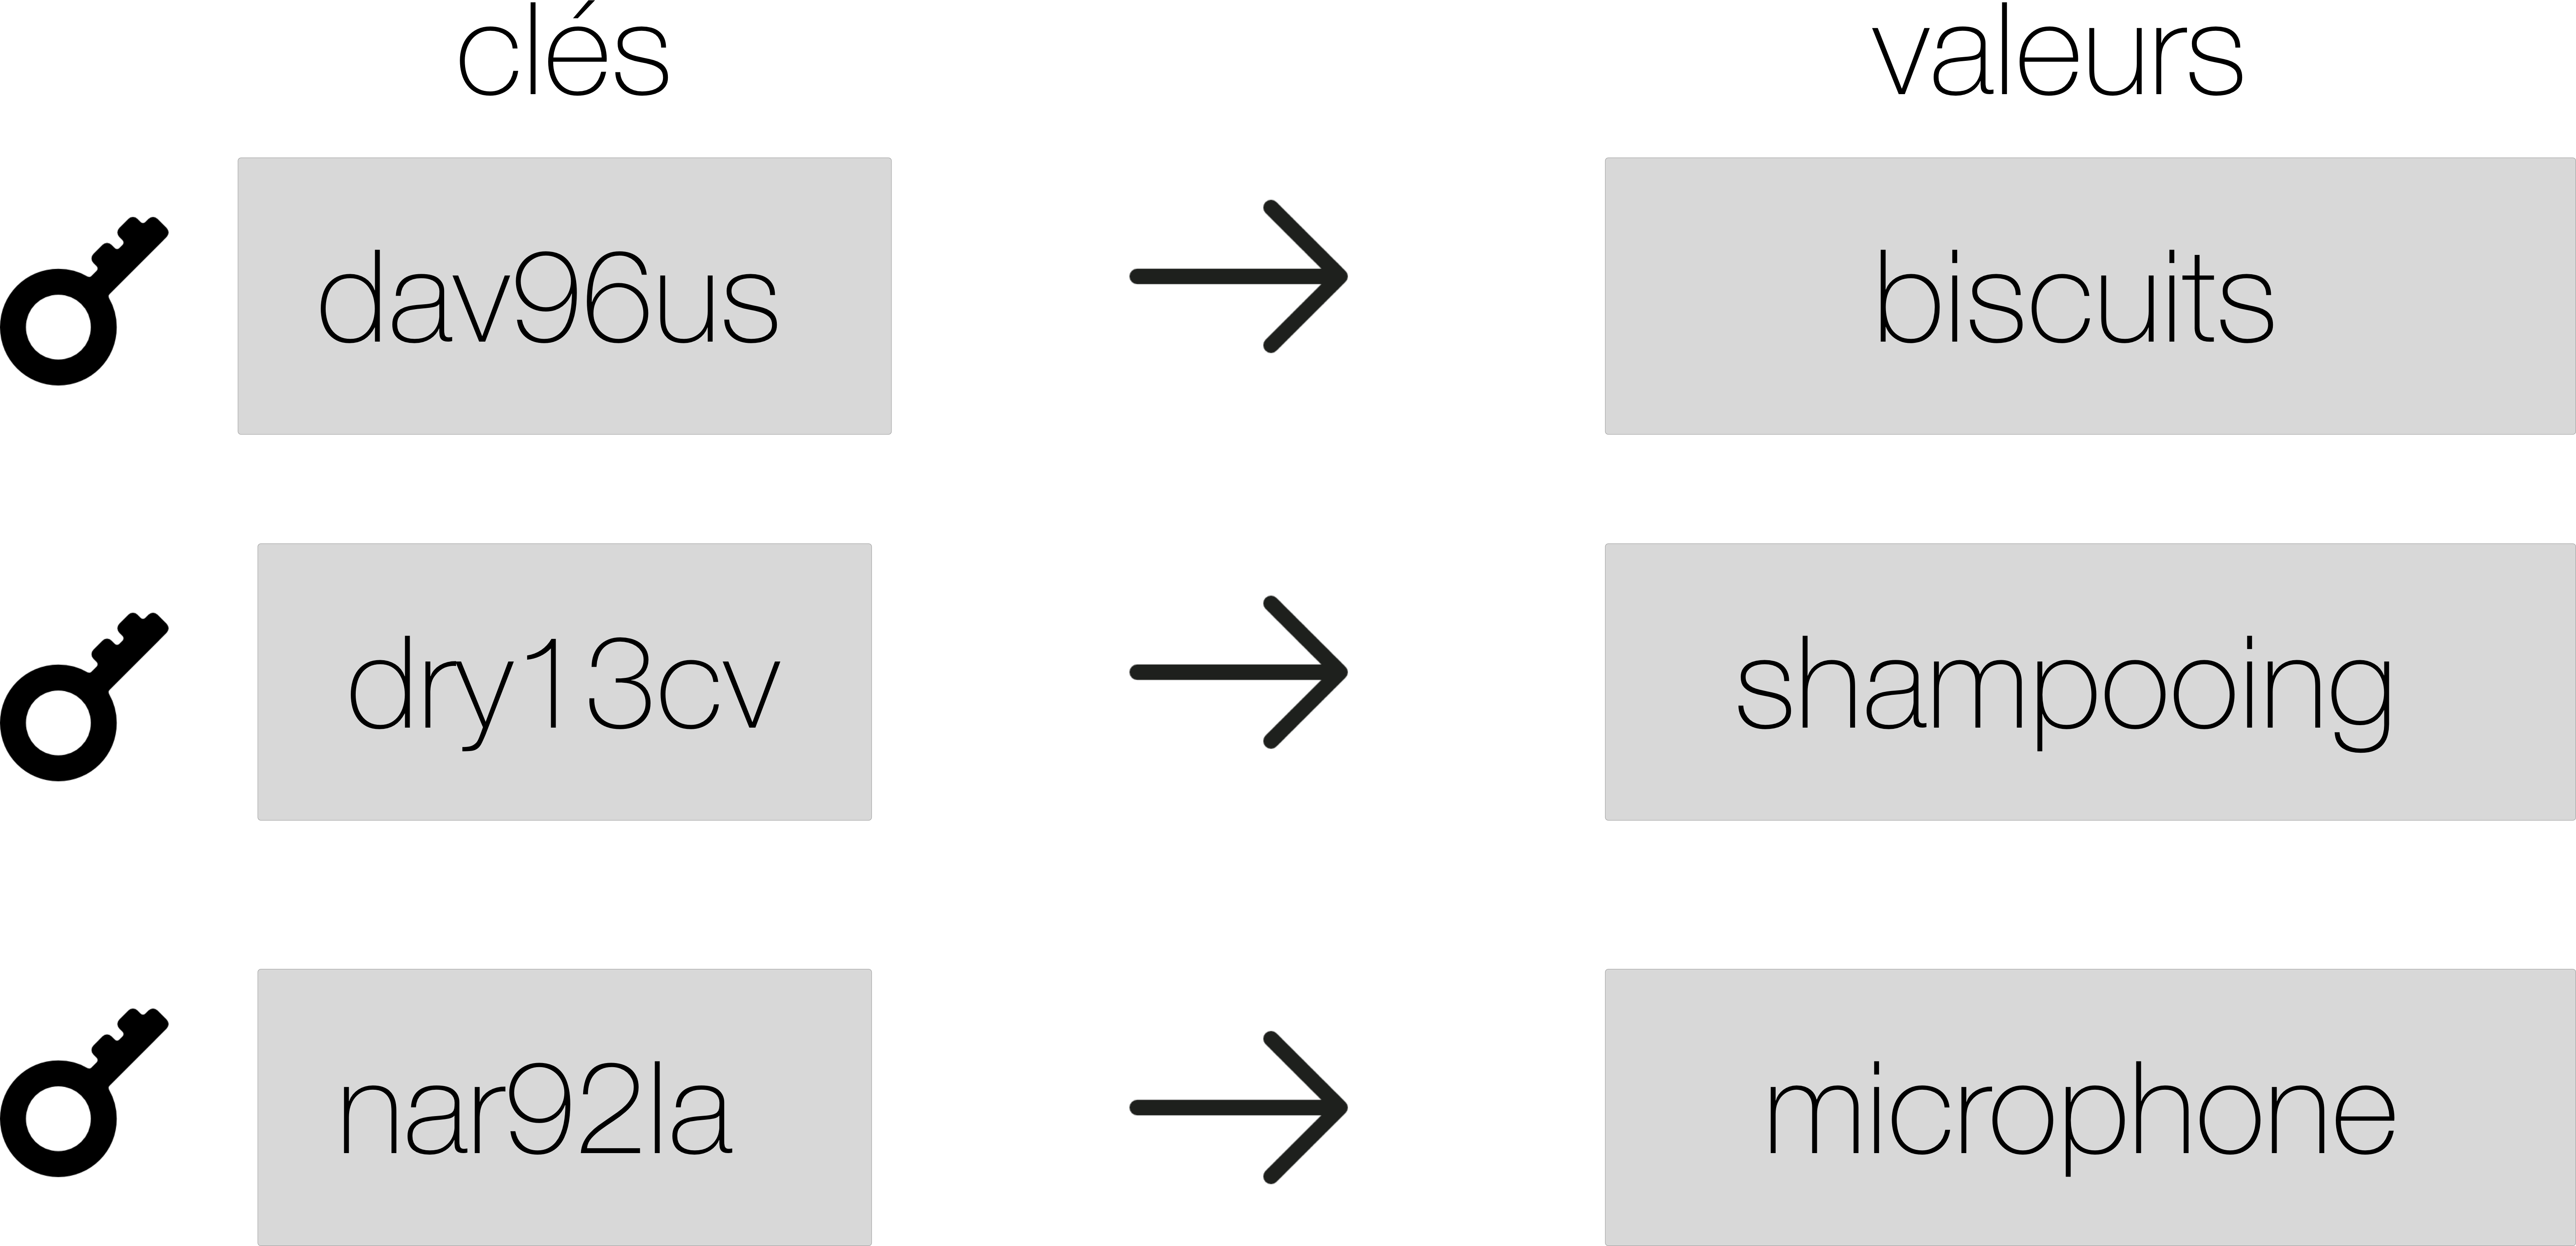
\includegraphics[width=0.6\textwidth]{key}
\caption{Entrepôt clé-valeur}
\end{figure}
Les opérations que l'on peut effectuer sur un tel entrepôt sont les suivantes : la récupération de la valeur pour une clé donnée, la mise à jour, la création ou la suppression d'une valeur pour une certaine clé. \par
Le modèle de cohérence à terme (\emph{éventuelle consistance}) est celui qui est retenu par une majorité des implémentations d'ECV. Le paramétrage fin de la consistance peut alors se faire au moyen de trois paramètres : 
\begin{itemize}
\item Le \textbf{facteur de réplication} qui définit le nombre N de nœuds sur lesquels doivent être répliquées les données.
\item Le \textbf{quorum d'écriture} W qui spécifie le nombre de nœuds dont on exige qu'ils notifient que les données ont été écrites avec succès pour considérer une opération d'écriture comme valide.
\item Le \textbf{quorum de lecture }R enfin, qui spécifie le nombre de nœuds minimal qu'il convient d'interroger être su d'obtenir la dernière version d'une donnée.
\end{itemize}
\vspace{0.4cm}
On parle de croissance forte lorsque $R+W>N$. Le contexte d'un ECV correspond donc à la valeur de la clé qui déterminera sur quel serveur est hébergée la valeur associée.
\par
Les implémentations des les plus répandues des entrepôts  clé-valeur sont \emph{Riak}, \emph{Redis}, \emph{Memcached DB} et \emph{DynamoDB} chez Amazon.
\par
Le stockage de données de session utilisateur est le cas typique d'utilisation d'un entrepôt clé-valeur. De manière similaire, le stockage des préférences ou des profils des utilisateurs ou encore les associations entre clients et paniers d'achats des sites d'e-commerce conviennent bien aux ECV. Ainsi, la structure des données en table de hachage les rend inadaptés pour retrouver des données à partir d'une valeur plutôt que d'une clé.
\paragraph{Les bases orientées documents}
Sur le plan conceptuel, les bases de données orientées document (BDOD) sont peu différent des ECV. En effet, une BDOD peut schématiquement se décrire comme un ECV dont les valeurs sont remplacées par des documents semi-structurés. En parlant de documents semi-structurés, on étend des documents auto descriptifs généralement écrits avec un format de type XML\footnote{XML : \emph{Extensible Markup Language}, ou en français le langage de balisage extensible est un métalangage informatique de balisage générique qui dérive du SGML}, JSON\footnote{JSON : \emph{JavaScript Object Notation}, est un format de données textuelles dérivé de la notation des objets du langage JavaScript.} ou similaire. Contrairement aux SGBDR qui requièrent que chaque enregistrement d'une table ait les mêmes colonnes, spécifiées par un schéma, rien n'exige que les documents stockés dans une BDOD aient tous le même format .\par
De ce point de vue, une BDOD est donc beaucoup plus flexible qu'un SGBDR dans la mesure où il est possible de modifier au coup par coup la strcutre d'un document sans avoir à respecter un schéma préétabli. Alors qu'une valeur non définie d'une colonne d'un enregistrement d'un SGBDR est représentée par la valeur NULL, un document d'une BDOD ne fera tout simplement pas figurer l'attribut en question.
Nous pouvons clarifier la relation entre SGBDR (\emph{Oracle}) et BDOD (\emph{MangoDB}) dans le tableau suivant : 
\begin{table}[]
\centering
\caption{Équivalences entre SGBDR et BDOD}
\begin{tabular}{c|c|}
\hline
\rowcolor[HTML]{C0C0C0} 
\textbf{BDOD}                                           & \textbf{SGBDR}          \\ \hline
\multicolumn{1}{|c|}{base de données}                   & schéma                  \\ \hline
\multicolumn{1}{|c|}{collection (de documents)}         & table                   \\ \hline
\multicolumn{1}{|c|}{document}                          & enregistrement          \\ \hline
\multicolumn{1}{|c|}{Id de document}                    & Id d'enregistrement     \\ \hline
\multicolumn{1}{|c|}{DBRef (référence entre documents)} & jointure (entre tables) \\ \hline
\end{tabular}
\end{table}
De plus, les BDOD offrent la possibilité d'examiner le contenu d'un document sans qu'il soit nécessaire pour autant de le récupérer en intégralité, en laquelle elles se distinguent des ECV. \par
La disponibilité des BDOD est généralement assurée par un mécanisme de réplication qui utilise un schéma de type maître-esclave. Les requêtes sont adressées par défaut au maître qui les redirige vers l'un des esclaves pour les opérations de lecture. La montée en charge se fait par simple ajout de nœuds esclaves. Si le maître tombe en panne, les nœuds esclaves procèdent à un vote pour élire un nouveau maître selon des critères de distance entre les nœuds ou de quantité de RAM disponible. L'application cliente n'a pas, quant à elle, à se soucier de se connecter à un nœud particulier ni à gérer les pannes de réseau. La technique de sharding est souvent utilisée par les BDOD, le système assurant une répartition équilibrée des données entre les nœuds en tenant compte constamment de la distance qui les sépare.\par
Les implémentations les plus répandues de BDOD à ce jour sont : \emph{MangoDB}, \emph{CouchDB}, \emph{RavenDB} et \emph{Lotus Notes}. \par
On peut être amené à utiliser des BDOD dans l'e-commerce dont les produits varient trop souvent pour être décrits au moyen d'un schéma stable.\\
Les applications qui manipulent naturellement des documents comme les systèmes de gestion de contenu ou les plateformes de blogs pourront elles aussi utiliser avec profit une BDOD.
\paragraph{Les bases orientées colonnes}
Au sein des bases de données orientées agrégats (BDOA), les bases orientées colonnes (BDOC) sont sans hésitation celles dont le modèle de données est le plus riche. Dû à la complexité d'aborder ce sujet avec toutes les variations d'un produit à un autre, c'est pour cette raison que nous allons nous concentrer sur le modèle de la BDOC \emph{Cassandra}, qui a un modèle particulièrement complet et clair. \par
Tout d'abord, nous allons établir dès le début le parallèle avec deux catégories de systèmes que nous avons déjà vu : les ECV et les SGBDR classiques.
\par
La première manière de définir, sur le plan conceptuel, une BDOC comme \emph{Cassandra} est qu'il s'agit d'un ECV dont les valeurs possèdent une structure bien particulière. Cette structure-là est celle de colonnes dont les noms peuvent être soit \emph{statiques}, ils sont alors partagés par tous les enregistrements d'une collection de colonnes, soit elles sont \emph{dynamiques}, c'est-à-dire qu'ils peuvent varier d'un enregistrement à l'autre au sein d'une telle collection.
\par
La présence de la possibilité d'avoir des colonnes dynamiques permet d'avoir des enregistrements avec colonnes différentes en type et en nombre, ce qui est impossible dans un SGBDR. Il existe un autre élément des structures qui est commun à beaucoup de BDOC, qui est la possibilité de regrouper entre elles des colonnes contenant des données sémantiquement liées. \\
L'enregistrement d'un client contiendra toutes ses commandes par exemple. Ces regroupements s'appellent des \textbf{super-colonnes}. Elles aussi peuvent à leur tour être statiques ou dynamiques. Selon que les colonnes ou les super-colonnes soient statiques ou dynamiques on peut alors construire quatre types de structures, que l'on appellera des \textbf{familles de colonnes}, appropriées à des situations différentes. Nous allons illustrer ces structures à l'aide de figures.
\begin{figure}[H]
\centering
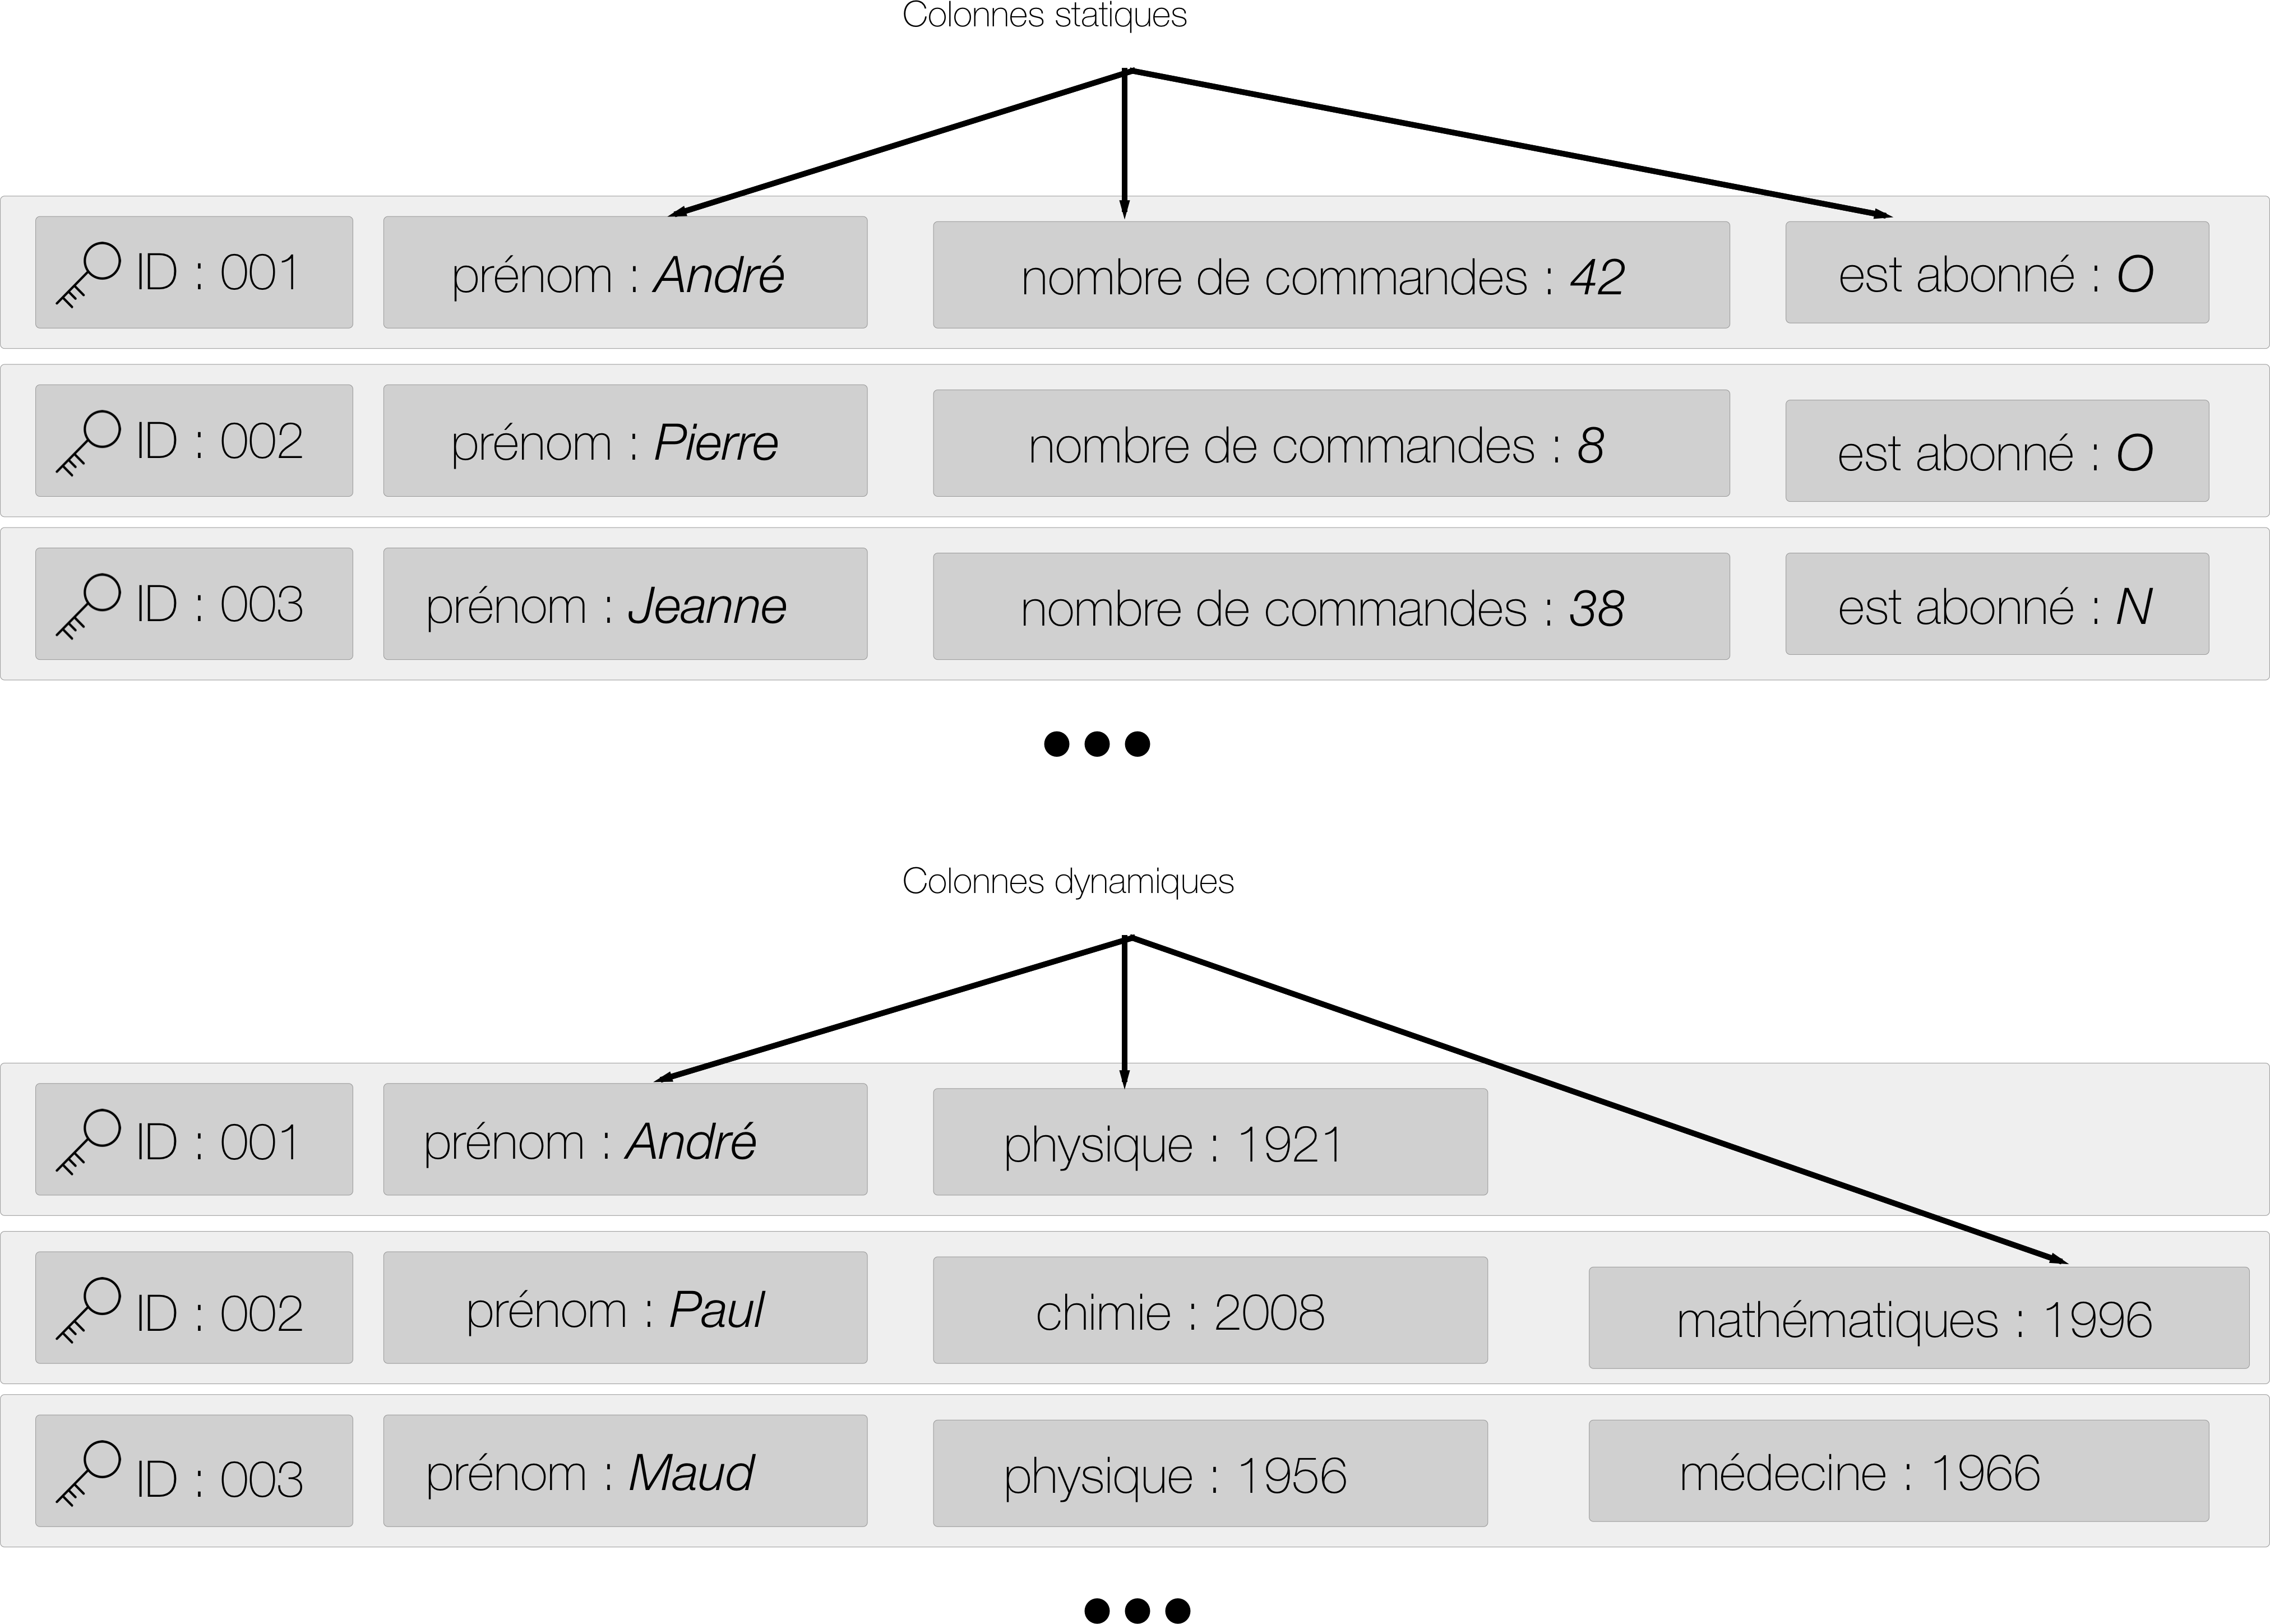
\includegraphics[width=0.8\textwidth]{colonnes}
\caption{Colonnes statiques et colonnes dynamiques}
\end{figure}
\begin{figure}[H]
\centering
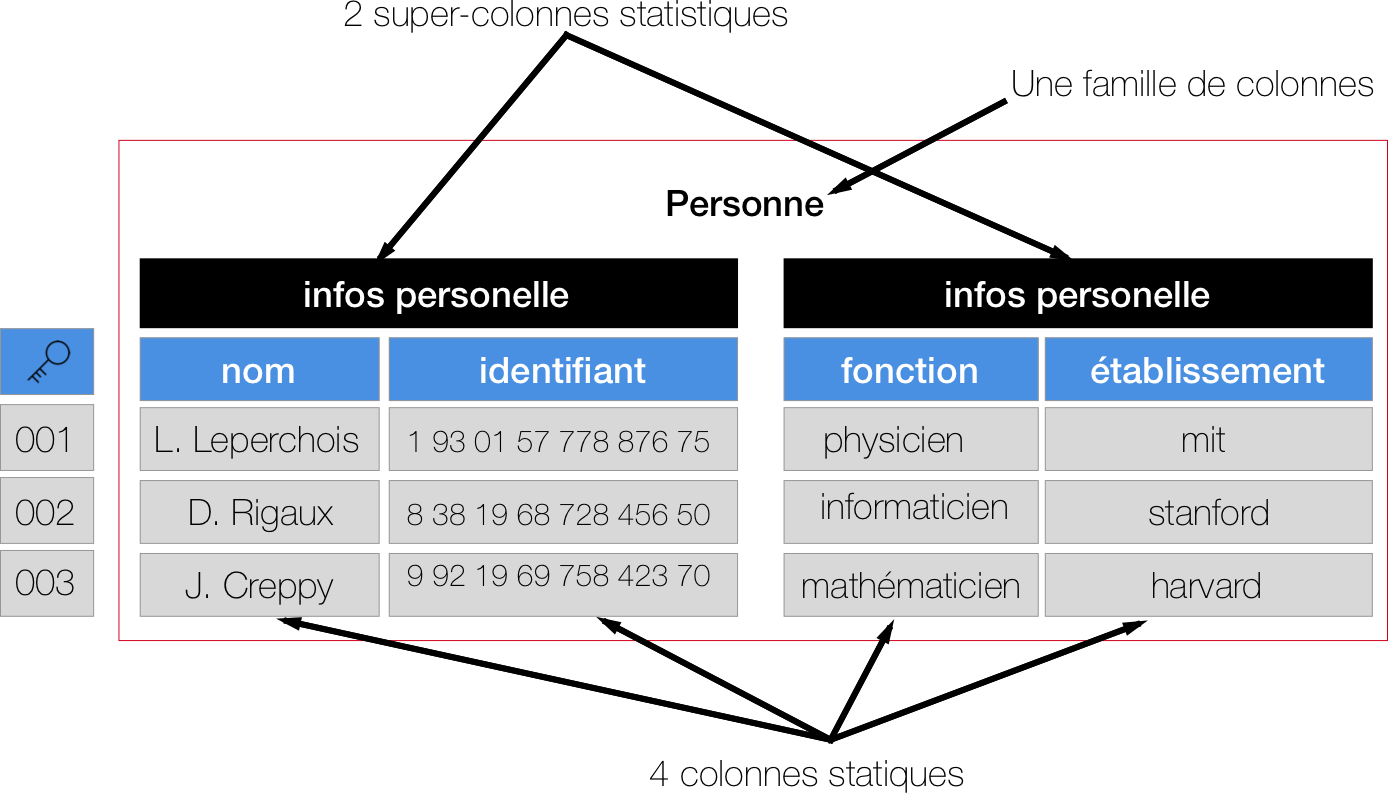
\includegraphics[width=0.8\textwidth]{super}
\caption{Super-colonnes}
\end{figure}
Nous allons résumer dans un tableau les analogies les plus pertinentes avec un SGBDR.
\begin{table}[]
\centering
\caption{Les analogies les plus pertinentes entre BDOC et SGBDR}
\begin{tabular}{c|c|}
\hline
\rowcolor[HTML]{C0C0C0} 
\textbf{BDOC (Cassandra)}                                                                                                                            & \textbf{SGBDR}                                                                                                   \\ \hline
\multicolumn{1}{|c|}{cluster}                                                                                                                        & instance de base de données                                                                                      \\ \hline
\multicolumn{1}{|c|}{keyspace}                                                                                                                       & base de données                                                                                                  \\ \hline
\multicolumn{1}{|c|}{famille de colonnes}                                                                                                            & table                                                                                                            \\ \hline
\multicolumn{1}{|c|}{enregistrement}                                                                                                                 & enregistrement                                                                                                   \\ \hline
\multicolumn{1}{|c|}{\begin{tabular}[c]{@{}c@{}}colonnes qui peuvent varier pour différents\\ enregistrements si elles sont dynamiques\end{tabular}} & \begin{tabular}[c]{@{}c@{}}colonnes qui sont les mêmes dans tous les \\ enregistrements d'une table\end{tabular} \\ \hline
\end{tabular}
\end{table}
Les BDOC les plus populaires à l'heure actuelle sont : \emph{Cassandra}, \emph{HBase}, \emph{Hypertable}, \emph{Amazon SimpleDB}.
\par
En effet, la flexibilité des BDOC en fait un choix idéal, par exemple, pour stocker des rapports d'erreurs issus de plusieurs applications dont chacune pourra utiliser le groupe de colonnes qui lui convient. L'utilisation d'une BDOC est particulièrement bien adaptée pour les blogs avec leurs publications, leurs liens, les rétroliens\footnote{Rétrolien : Un système de liens inter-blogs semi-automatisé. Il permet aux auteurs de relier des billets de blogs différents et parlant du même sujet, ou ce faisant référence.} Ainsi que les commentaires associés. De plus, les systèmes de comptage de nombre de visites peuvent tirer profit de la classification à deux niveaux, par site et par page, que permet le modèle des colonnes dynamiques.
\paragraph{Les bases de données orientées graphes}
Il existe de nombreuses situations comme les réseaux sociaux, où il s'agit de relier des entités par différentes relations, elles-mêmes dotées d'attributs et d'un sens de navigation. Telle personne \og aime \fg , \og connaît \fg ou \og font partie du cercle professionnel \fg de telles autres. Malgré leur nom, les SGBDR (où le \og R \fg = relationnel) ne sont pas bien adaptés pour parcourir rapidement un graphe. Un SGBDR n'est pas bien adapté pour décrire des relations complexes comme celles qui lient un client à ses commandes, par exemple. Mais, dès que le nombre de liens à parcourir excède un ou deux, la nécessité de définir à chaque fois des clés étrangères et d'effectuer de nombreuses jointures pénalise les performances au point de rendre cette approche impraticable.
\par
Par dessus les limitations des SGBDR, il faut également ajouter l'impossibilité pure et simple d'effectuer certaines opérations naturelles sur un graphe. Parcourir l'intégralité d'un graphe ou trouver un chemin entre deux nœuds vérifiant certaines contraintes sont deux exemples élémentaires. Les bases de données orientées graphes ont été conçues pour répondre spécifiquement à cette catégorie de besoins. Elles permettent dans un premier temps de créer des nœuds puis, indépendamment, de créer des associations entre eux et de les modifier par la suite.\par
Beaucoup de BDOG ne prennent pas en charge la distribution des nœuds de données sur un cluster et l'ACIDité n'est assurée qu'au sein d'un seul serveur. 
\begin{figure}[H]
\centering
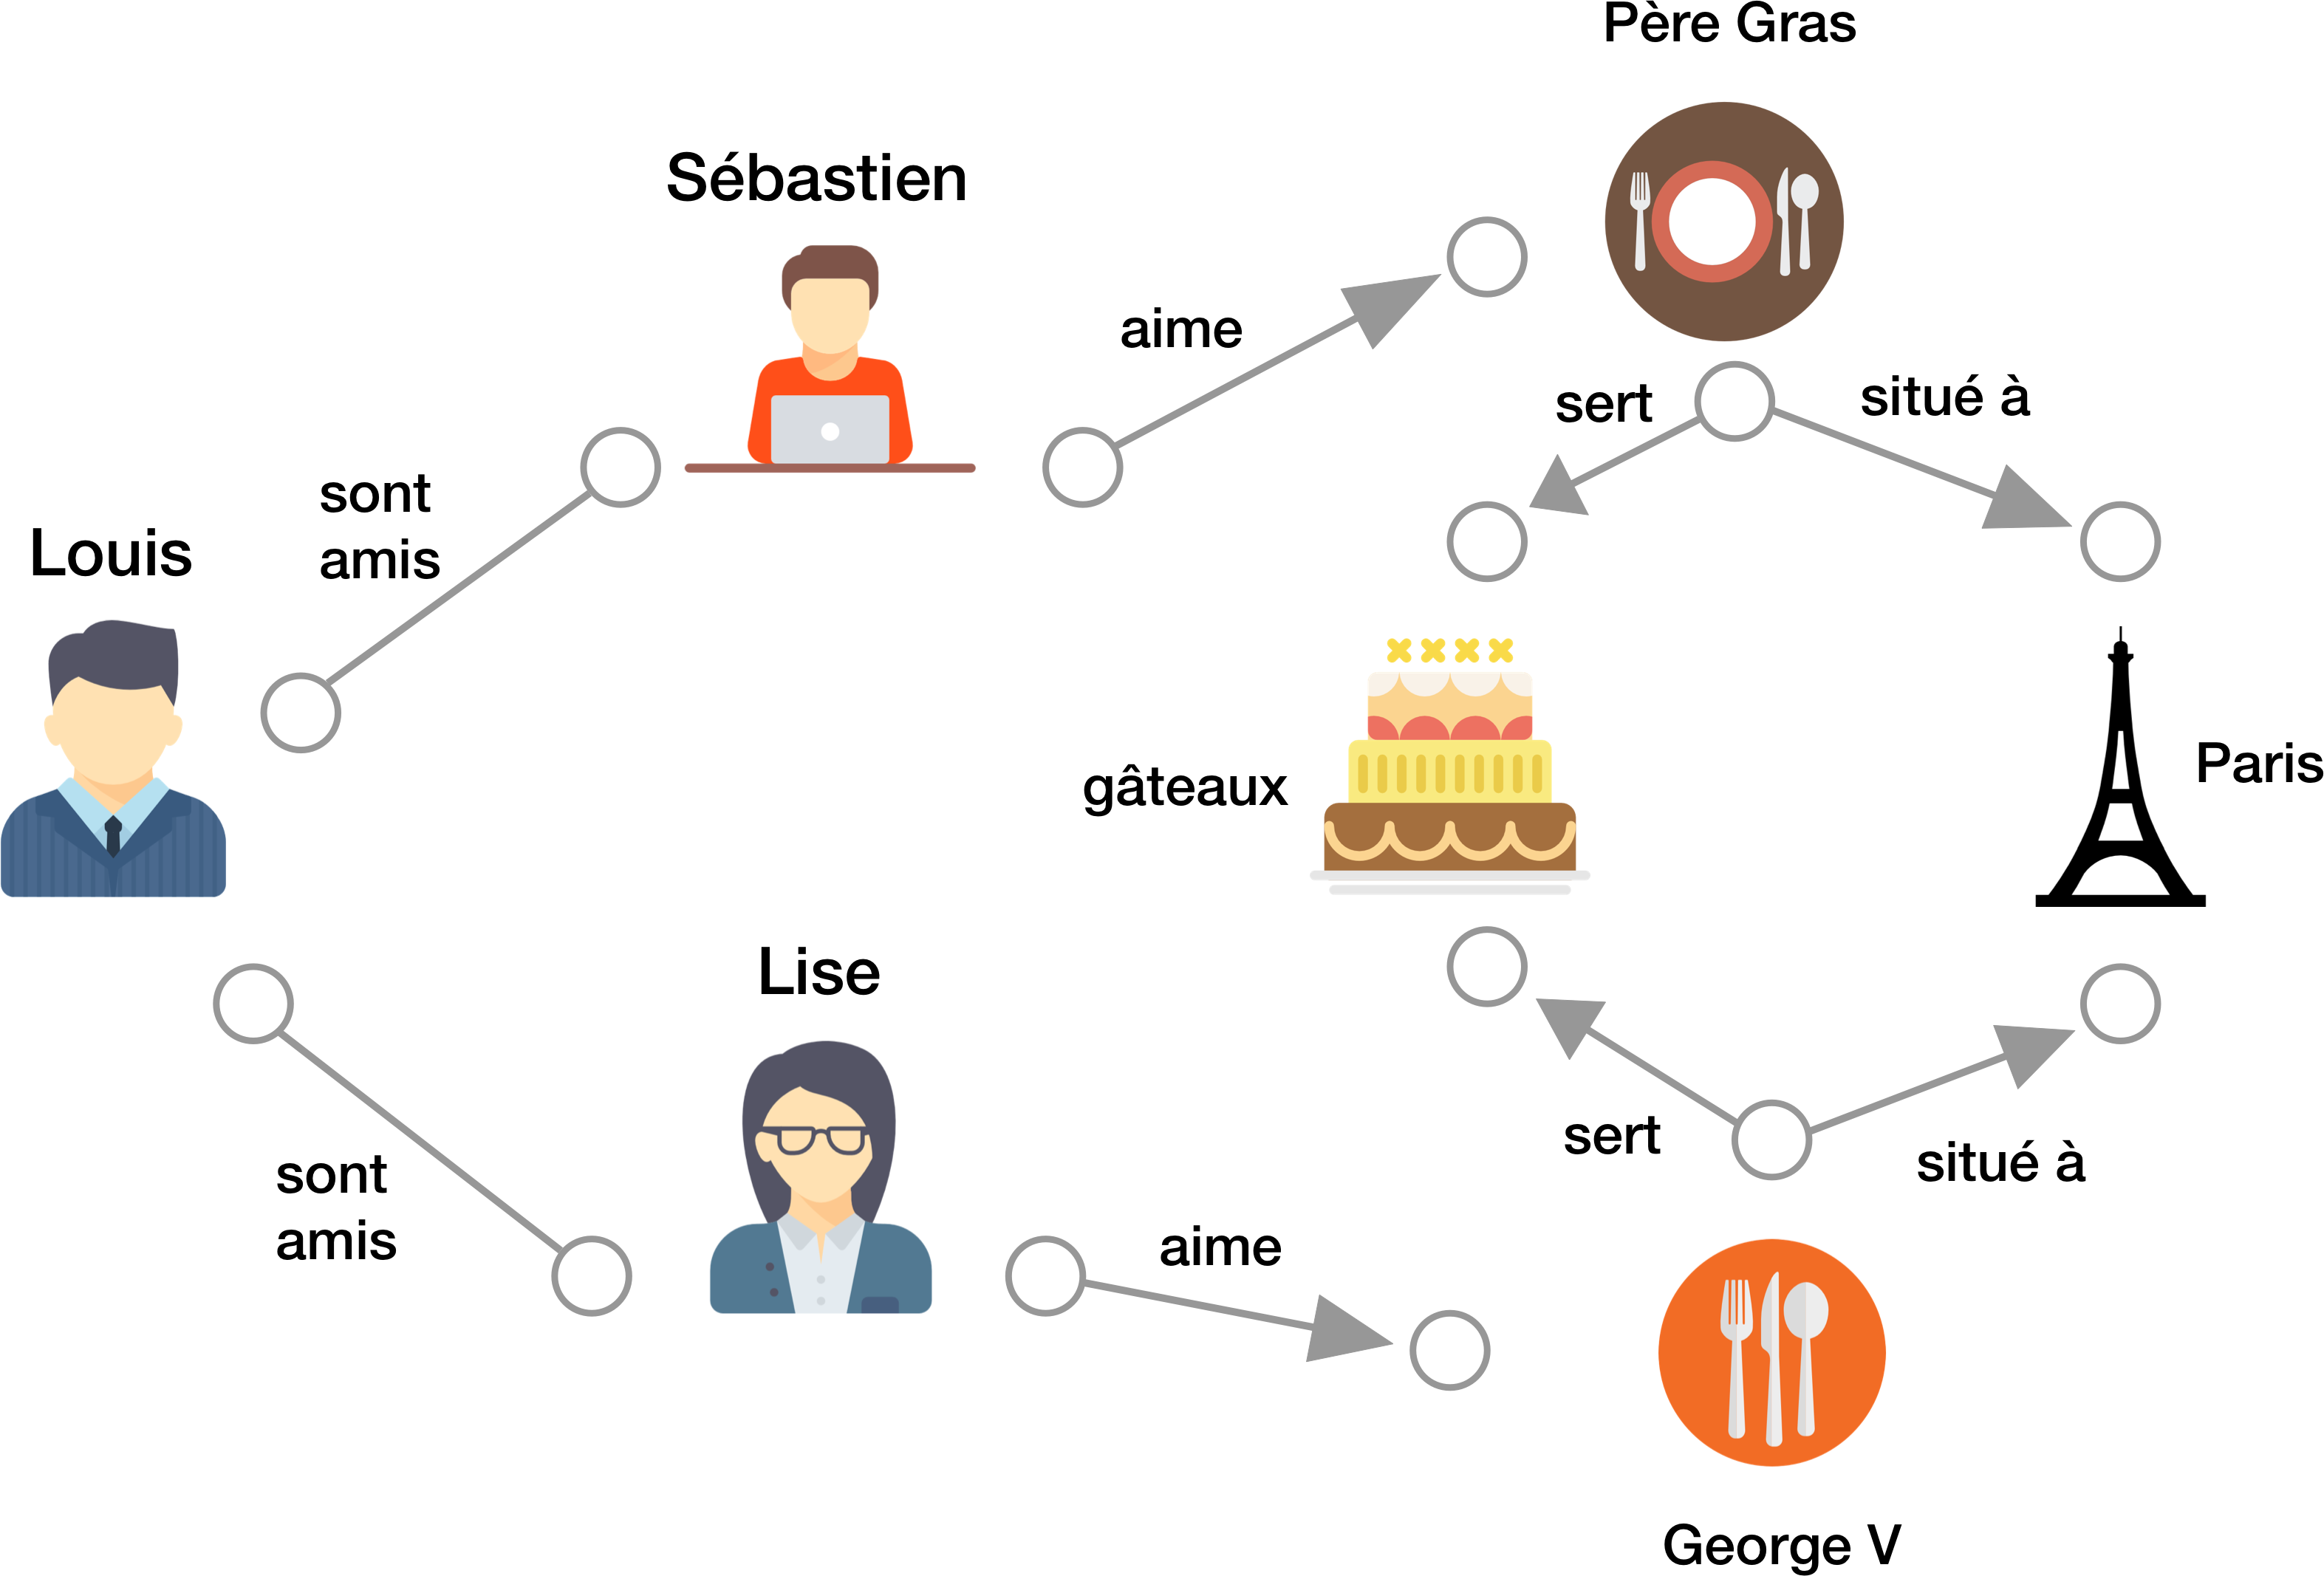
\includegraphics[width=0.9\textwidth]{graph}
\caption{Un exemple de graphe qui relie des individus, des services et des lieux géographiques}
\end{figure}
En quelque sorte, la stratégie mise en œuvre dans une BDOG est à l'opposé de celle utilisée par BDOA. Même si ces dernières regroupent des données au sein d'agrégats, les BDOG les éclatent autant que possible dans un graphe. \par
Parmis les BDOG les plus utilisés aujourd'hui on retrouve : \emph{Neo4J}, \emph{Infinite Graph} et \emph{OrientDB}.
\par
Tous les domaines de métiers qui s'expriment naturellement à l'aide de graphes sont éligibles à l'utilisation d'une BDOG. Ils sont particulièrement utiles dans les situations où différentes catégories de liens expriment des appartenances à certains groupes sociaux ou géographiques. Dans ces derniers cas, l'un des attributs des liens sera la distance qui sépare les nœuds qu'ils connectent. Il faut savoir que tous les systèmes de recommandation ou de détection de fraude qui doivent tenir compte d'une certaine proximité, que ce soit géographie, sociale ou autre pourront tirer profit d'un BDOG.
\subsubsection{L'algorithme MapReduce et le framework Hadoop}
MapReduce est un modèle de programmation récent, qui a permis d'automatiser le déploiement de traitements massivement parallèles sur de clusters de centaines ou de milliers de serveurs peu coûteux. \par
Dans le contexte du Big Data, l’algorithme MapReduce à lui seul ne serait pas d'une grande utilité sans une infrastructure logicielle dédiée, c'est donc pour cela que nous présenterons les grandes lignes du fonctionnement de Hadoop, qui est à ce jour la principale implémentation open source d'une telle infrastructure. \par
Une des possibilités pour passer à l'échelle consiste à les paralléliser sur un cluster de plusieurs centaines ou milliers de machines. Malheureusement, cette mise en parallèle est en règle générale une tâche qui est très difficile à réaliser qui nécessite un savoir-faire spécialisé et une longue phase de conception. De plus, dans les situations où un code non parallélisé existe déjà, un important travail de réécriture est le plus souvent nécessaire. \par

Un des progrès les plus significatifs dans l’automatisation de la parallélisation est venu de travaux de recherches effectués par Google pour les besoins de son moteur de recherche. 
En effet, au début des années 2000, des centaines de processus parallèles avaient été conçus par les ingénieurs de Mountain View\footnote{La Silicon Valley} pour traiter les quantités phénoménales d’information récoltées par les \emph{web crawlers}\footnote{Web Crawler (en français \og robot d'indexation \fg)  est un logiciel qui explore automatiquement le Web.} du moteur de recherche : création d'annuaires inversés (liste de documents contenant certains mots clés), analyse des graphes de liens entre documents, identification des requêtes les plus fréquentes, etc. Bien que tous ces processus aient été conçus à l’origine par des équipes différentes, les ingénieurs se sont ensuite aperçus que beaucoup de ces programmes mettaient en œuvre une stratégie similaire pour paralléliser les traitements.
\par
Il s'agit de ce pattern de répartition des tâches que nous allons décrire dans cette et que l’on appelle MapReduce. À lui tout seul, la logique des traitements de MapReduce ne serait pas d'une grande utilité, du moins dans un contexte Big Data, sans une infrastructure logicielle qui prend en charge la complexité liée à la distribution des traitements, à la réplication des données et à la tolérance aux pannes. C'est pour cela que nous présenterons les grandes lignes du fonctionnement de Hadoop, qui est à ce jour l’implémentation open source de référence d'un tel framework d'exécution distribuée du pattern MapReduce. Nous verrons par la suite les principaux éléments de l'écosystème Hadoop.
\par
Pour être plus précise, la définition des abstractions MapReduce a été inspirée non seulement par une synthèse d’expériences chez Google mais aussi par des travaux antérieurs dans le domaine de la programmation fonctionnelle.
\par
Le pattern de MapReduce a été décrit pour la première fois en 2004 dans un article rédigé par deux ingénieurs de Google. Sur un plan intuitif, MapReduce part de l'observation que, dans de nombreuses situations, la mise en parallèle d'un traitement peut s'effectuer au moyen de seulement deux types d'opérations, possédant une structure bien précise.
\par
La première contrainte rencontrée par l'algorithme MapReduce est que les données d'entrée doivent être organisées comme une liste de couples clé-valeur, analogues à celles qui sont stockées dans les ECV\footnote{ECV : entrepôt clé-valeur} ou les BDOD\footnote{Base de données orientée documents}. En pratique, cette liste peut être très volumineuse, sa taille pouvant être chiffrée en téraoctets ou même en pétaoctets. \par
Cette liste en entrée est tout d'abord scindée en plusieurs lots, grâce au framework. Par la suite, chaque lot est attribué à une des machines appelées \emph{mapper}.
\begin{figure}[H]
\centering
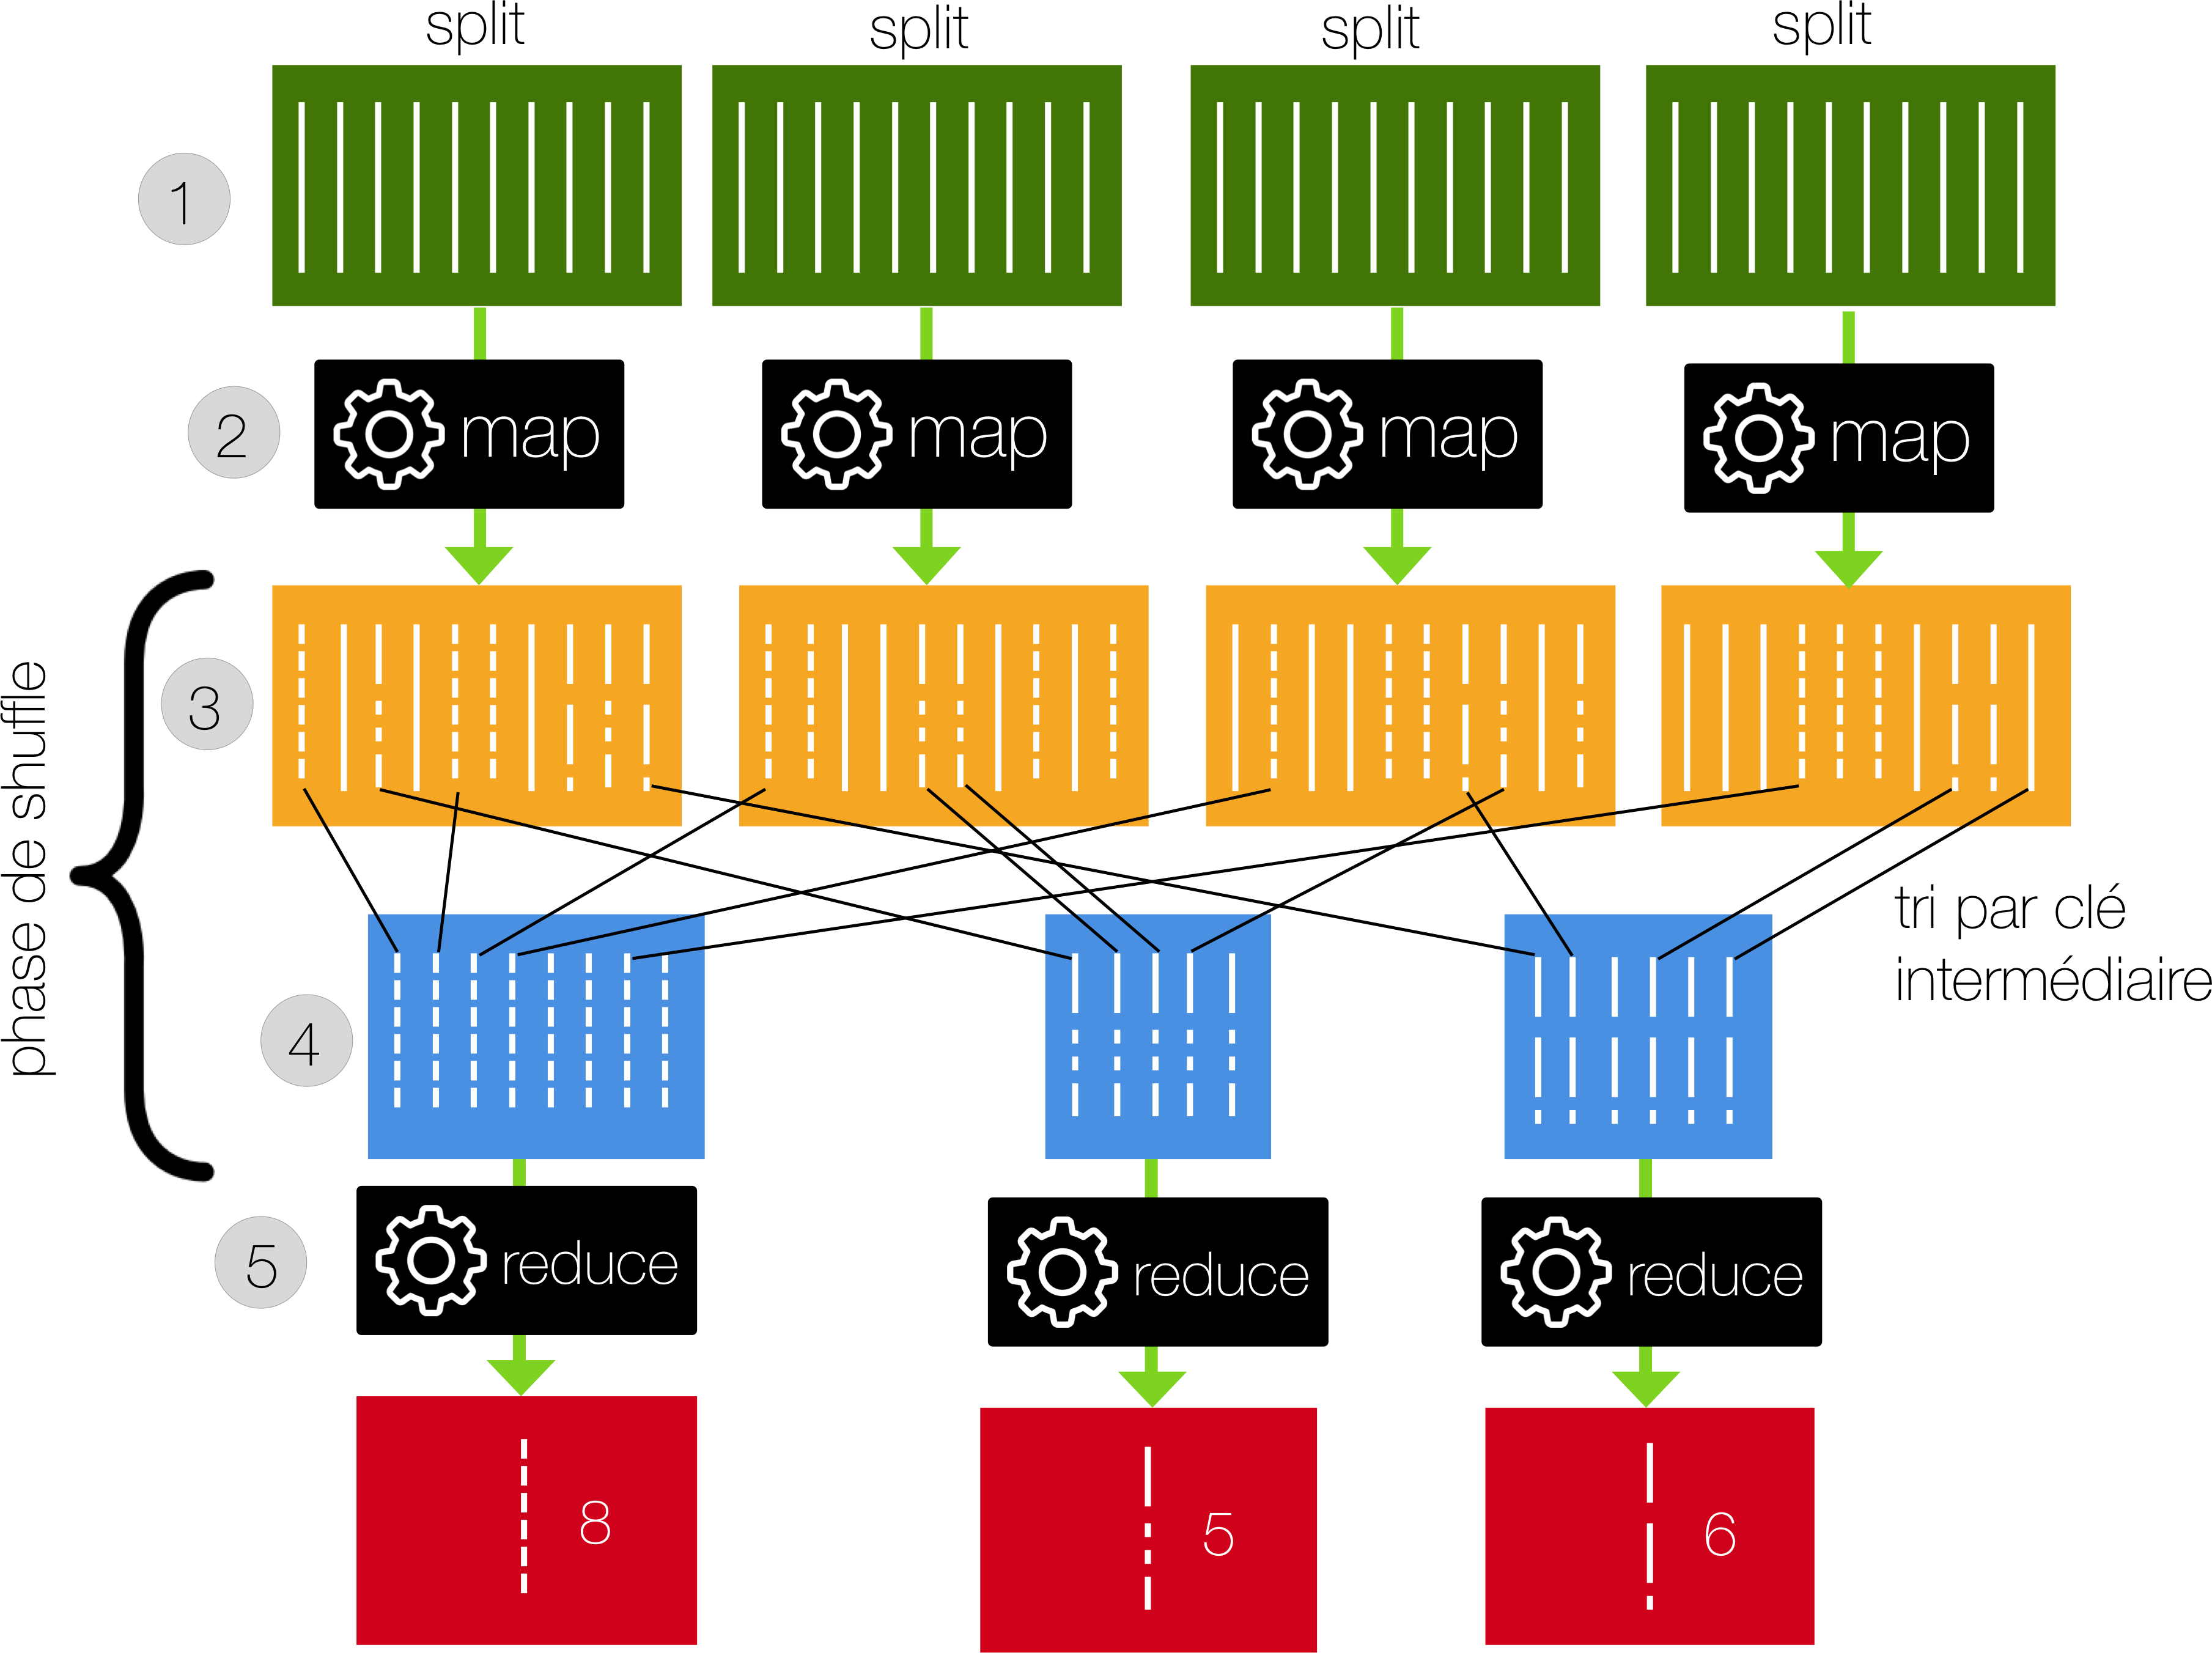
\includegraphics[width=1\textwidth]{mr}
\caption{Les données initiales sont scindées en lots. Chaque lot, aussi appelé splits, est confié à un mapper qui évalue la fonction map sur chaque enregistrement. Les listes obtenues en sortie des mappers sont concaténées, classées par valeur de la clé intermédiaire et scindées en lots par le framework. C'est la phase dite du shuffle. Les reducers évaluent la fonction reduce sur des listes de valeurs associées à une même valeur de clé intermédiaire.}
\end{figure}
\begin{itemize}
\item Tout d'abord, ces mappers exécutent une opération dite \og map \fg  sur chacun des enregistrements du lot qui leur a été confiée. Chaque invocation de cette opération map retourne alors une liste de clés-valeurs intermédiaires que l'on peut envisager comme un résultat intermédiaire du calcul à effectuer sur la liste complète.
\end{itemize}
\begin{req}
Les traitements map doivent être impérativement indépendant puisque c'est elle qui autorise la mise en parallèle de leur exécution, soit sur des machines différentes, soit au sein de processus distincts.
\end{req}
\begin{itemize}
\item Puis, une fois que tous les mappers ont tous fini leur tâche, les fonctions \og reduce \fg , exécutées par des reducers, agrègent systématiquement toutes les valeurs intermédiaires associées à une même clé intermédiaire. Pour cela, le framework fusionne au préalable les listes intermédiaires en sortie des mappers, les trie selon la valeur des clés, les répartit en lots puis enfin les achemine vers les reducers. Chaque lot sera assigné à un seul reducer et les lots sont constitués de telle manière que  toutes les valeurs associées à une même clé figurent dans le même lot.
\end{itemize}
Ainsi, l’opération \og reduce\fg  peut donc être envisagée comme une opération de recombinaison ou d'agrégation des résultats partiels obtenus par les mappers lors de la première phase.
\subsubsection{L'écosystème Hadoop}
\begin{figure}[H]
\centering

\includegraphics[width=0.8\textwidth]{hadoop}
\end{figure}
Hadoop était initialement conçu pour fournir un environnement d'exécution distribué pour le pattern MapReduce, mais Hadoop se diversifie aujourd'hui en une multitude de projets satellites. Nous allons maintenant présenter les principaux systèmes qui constituent Hadoop ainsi que ceux qui étendent ses fonctionnalités.
\subsubsection{Distribution ou package}
Comme vu précédemment Hadoop est un projet open source de la fondation Apache dont l'objectif principal est de développer des outils facilitant la construction d'application scalables distribuée sur des clusters de serveurs bon marché. Dans sa version originale, Hadoop était conçu comme un framework \footnote{framework : En programmation informatique, ceci est un ensemble cohérent de composants logiciels structurels, qui sert à créer les fondations ainsi que les grandes lignes de tout ou d'une partie d'un logiciel.} d'exécution distribuée pour le pattern MapReduce. \par
Hadoop n'est pas une exception, même s'il est open source cela et que les briques logicielles soient gratuites, cela n'implique en aucun cas la gratuité du service qu'elles apportent. \\
Le niveau de technicité requis, qu'il s'agisse de déployer le framework de Hadoop sur un cluster, de le configurer ou de l'intégrer est particulièrement important.  Il existe deux raisons principales à cela : 
\begin{itemize}
\item L'installation de Hadoop dans un environnement distribué est une tâche complexe qui exige l'écriture de nombreux fichiers de configuration, de scripts et qui demande de spécifier de nombreuses variables d'environnement.
\item Les différentes briques logicielles du projet Hadoop évoluent sans cesse et existent donc en plusieurs versions (\emph{releases}) qui ne sont pas forcément compatibles entre elles. 
\end{itemize} 
Il existe cependant plusieurs solutions pour surmonter ces difficultés, sans pour autant avoir à devenir soi-même un expert.
\par
La toute première solution consiste à utiliser ce qu'on appelle une \textbf{distribution Hadoop}. En effet, une distribution est un ensemble cohérent des différentes briques qui constituent l'écosystème Hadoop packagées par un fournisseur. Ce fournisseur peut également vendre ses propres outils graphiques pour simplifier le déploiement, la configuration et le monitoring du framework (GUI). Les trois principales distributions sont aujourd'hui celles de \emph{Cloudera}, de \emph{Hortonworks} et de \textit{MapR}. Pour les solutions en mode \textit{cloud}, il y a \textit{Elastic MapReduce} (EMR) d'Amazon, qui pour l'instant, fait référence.\par
La deuxième possibilité est d'utiliser un \textbf{package} Big Data. Un package comme celui-ci s'appuie sur une ou plusieurs distributions Hadoop, auxquelles viennent s'ajouter des outils de productivité comme :
\begin{itemize}
\item des \textbf{plugin} intégrés aux environnements de développement comme Eclipse ;
\item des \textbf{générateurs de code} qui produisent du code MapReduce à partir d'une représentation graphique des services ;
\item des \textbf{connecteurs} capables de récupérer l'information à partir de supports variés, qu'il s'agisse de SGBDR, de systèmes NoSQL ou de média sociaux comme Twitter ou Facebook, et de les charger dans Hadoop.
\end{itemize}
De plus, certains éditeurs comme Oracle par exemple proposent des appliances qui combinent logiciels et matériels.
\subsubsection{Un monde de compromis}
Au jour d'aujourd'hui, le système qui s'occupait de l'interrogation en langage naturel en temps réel d'un pétaoctet\footnote{$1 \text{pétaoctet} = 10^{15} \text{octets}$} de données non structurées n'est pas encore possible. C'est pour cela que les différents systèmes qui cherchent à améliorer ou à concurrencer Hadoop sont tous contraints d'effectuer certains compromis sur différents paramètres :
\begin{itemize}
\item le temps de réponse du système,
\item la flexibilité du modèle de données que l'on peut interroger,
\item la complexité du langage de requête,
\item la compatibilité avec les systèmes existants.
\end{itemize}
\par
Pour y voir plus clair, il est important  de garder à l'esprit qu'il existe très schématiquement trois types de besoins en analyse de données selon les temps de réponse attendus ou tolérables :
\begin{itemize}
\item Des traitements de type ETL sur de très grands volumes de données (allant jusqu'à plusieurs pétaoctets) qui peuvent donc être effectués en mode batch\footnote{mode batch : En informatique est un enchaînement automatique d'une suite de commandes sur un ordinateur sans intervention d'un opérateur}. Cependant, la complexité du code n'est pas un enjeu en l'occurrence.
\item Des analyses exploratoires et interactives effectuées par des data scientistes ou des experts métiers. L'aspect itératif est ici essentiel, de même que la possibilité d'interroger le système au moyen d'un langage standard comme le SQL. Les temps de réponse de l'ordre de quelques dizaines de secondes sont en revanche encore acceptables.
\item les systèmes qui exigent un délai de réponse inférieur à la seconde comme ceux qu'utilisent des agents commerciaux en contact direct avec une clientèle à laquelle ils doivent une réponse sur-le-champ.
\end{itemize}
\subsubsection{Les services autour de Hadoop}
Pour pouvoir utiliser Hadoop correctement, il existe de nombreux guides qui proposent leurs services : 
\begin{itemize}
\item \textbf{Communautés open source} - La communauté Apache Hadoop, très active, offre de nombreux forums, wiki, FAQ et blogs où s'échangent les dernières informations techniques sur la plateforme. Si l'information est naturellement gratuite, elle s'adresse toutefois à une audience de développeurs chevronnés et d'administrateurs dotés d'un fort niveau technique et rompus aux codes des communautés de logiciel libre.
\item \textbf{Intégrateurs} - Les intégrateurs et les fournisseurs de distribution Hadoop comme \textit{Cloudera}, \textit{Hortonworks} ou \textit{MapR} ou encore des éditeurs comme \textit{Talend} ou \textit{IBM}. Ces sociétés offrent un accès payant à guichet unique pour toutes les problématiques liées à Hadoop : conseil technologique, recherche de cas d'utilisation Big Data, assistance au déploiement, à l'intégration et à la personnalisation de produits open source.
\item \textbf{Éditeurs} - Ce sont ceux qui offrent des extensions propriétaires pour la plateforme Hadoop. Le domaine d'activité de prédilection de ces sociétés est la visualisation des données, l'analyse exploratoire et le machine learning. Une société leader dans ce domaine est \textit{Karmasphere}. Elle propose un environnement collaboratif exclusivement fait pour l'analyse itérative et à la visualisation de données traitées dans Hadoop.
\end{itemize}
\subsubsection{Les composants de Apache Hadoop}
Nous allons maintenant voir les principaux modules qui constituent le projet Hadoop ainsi que d'autres projets Apache qui lui sont directement reliés.
\begin{figure}[H]
\centering
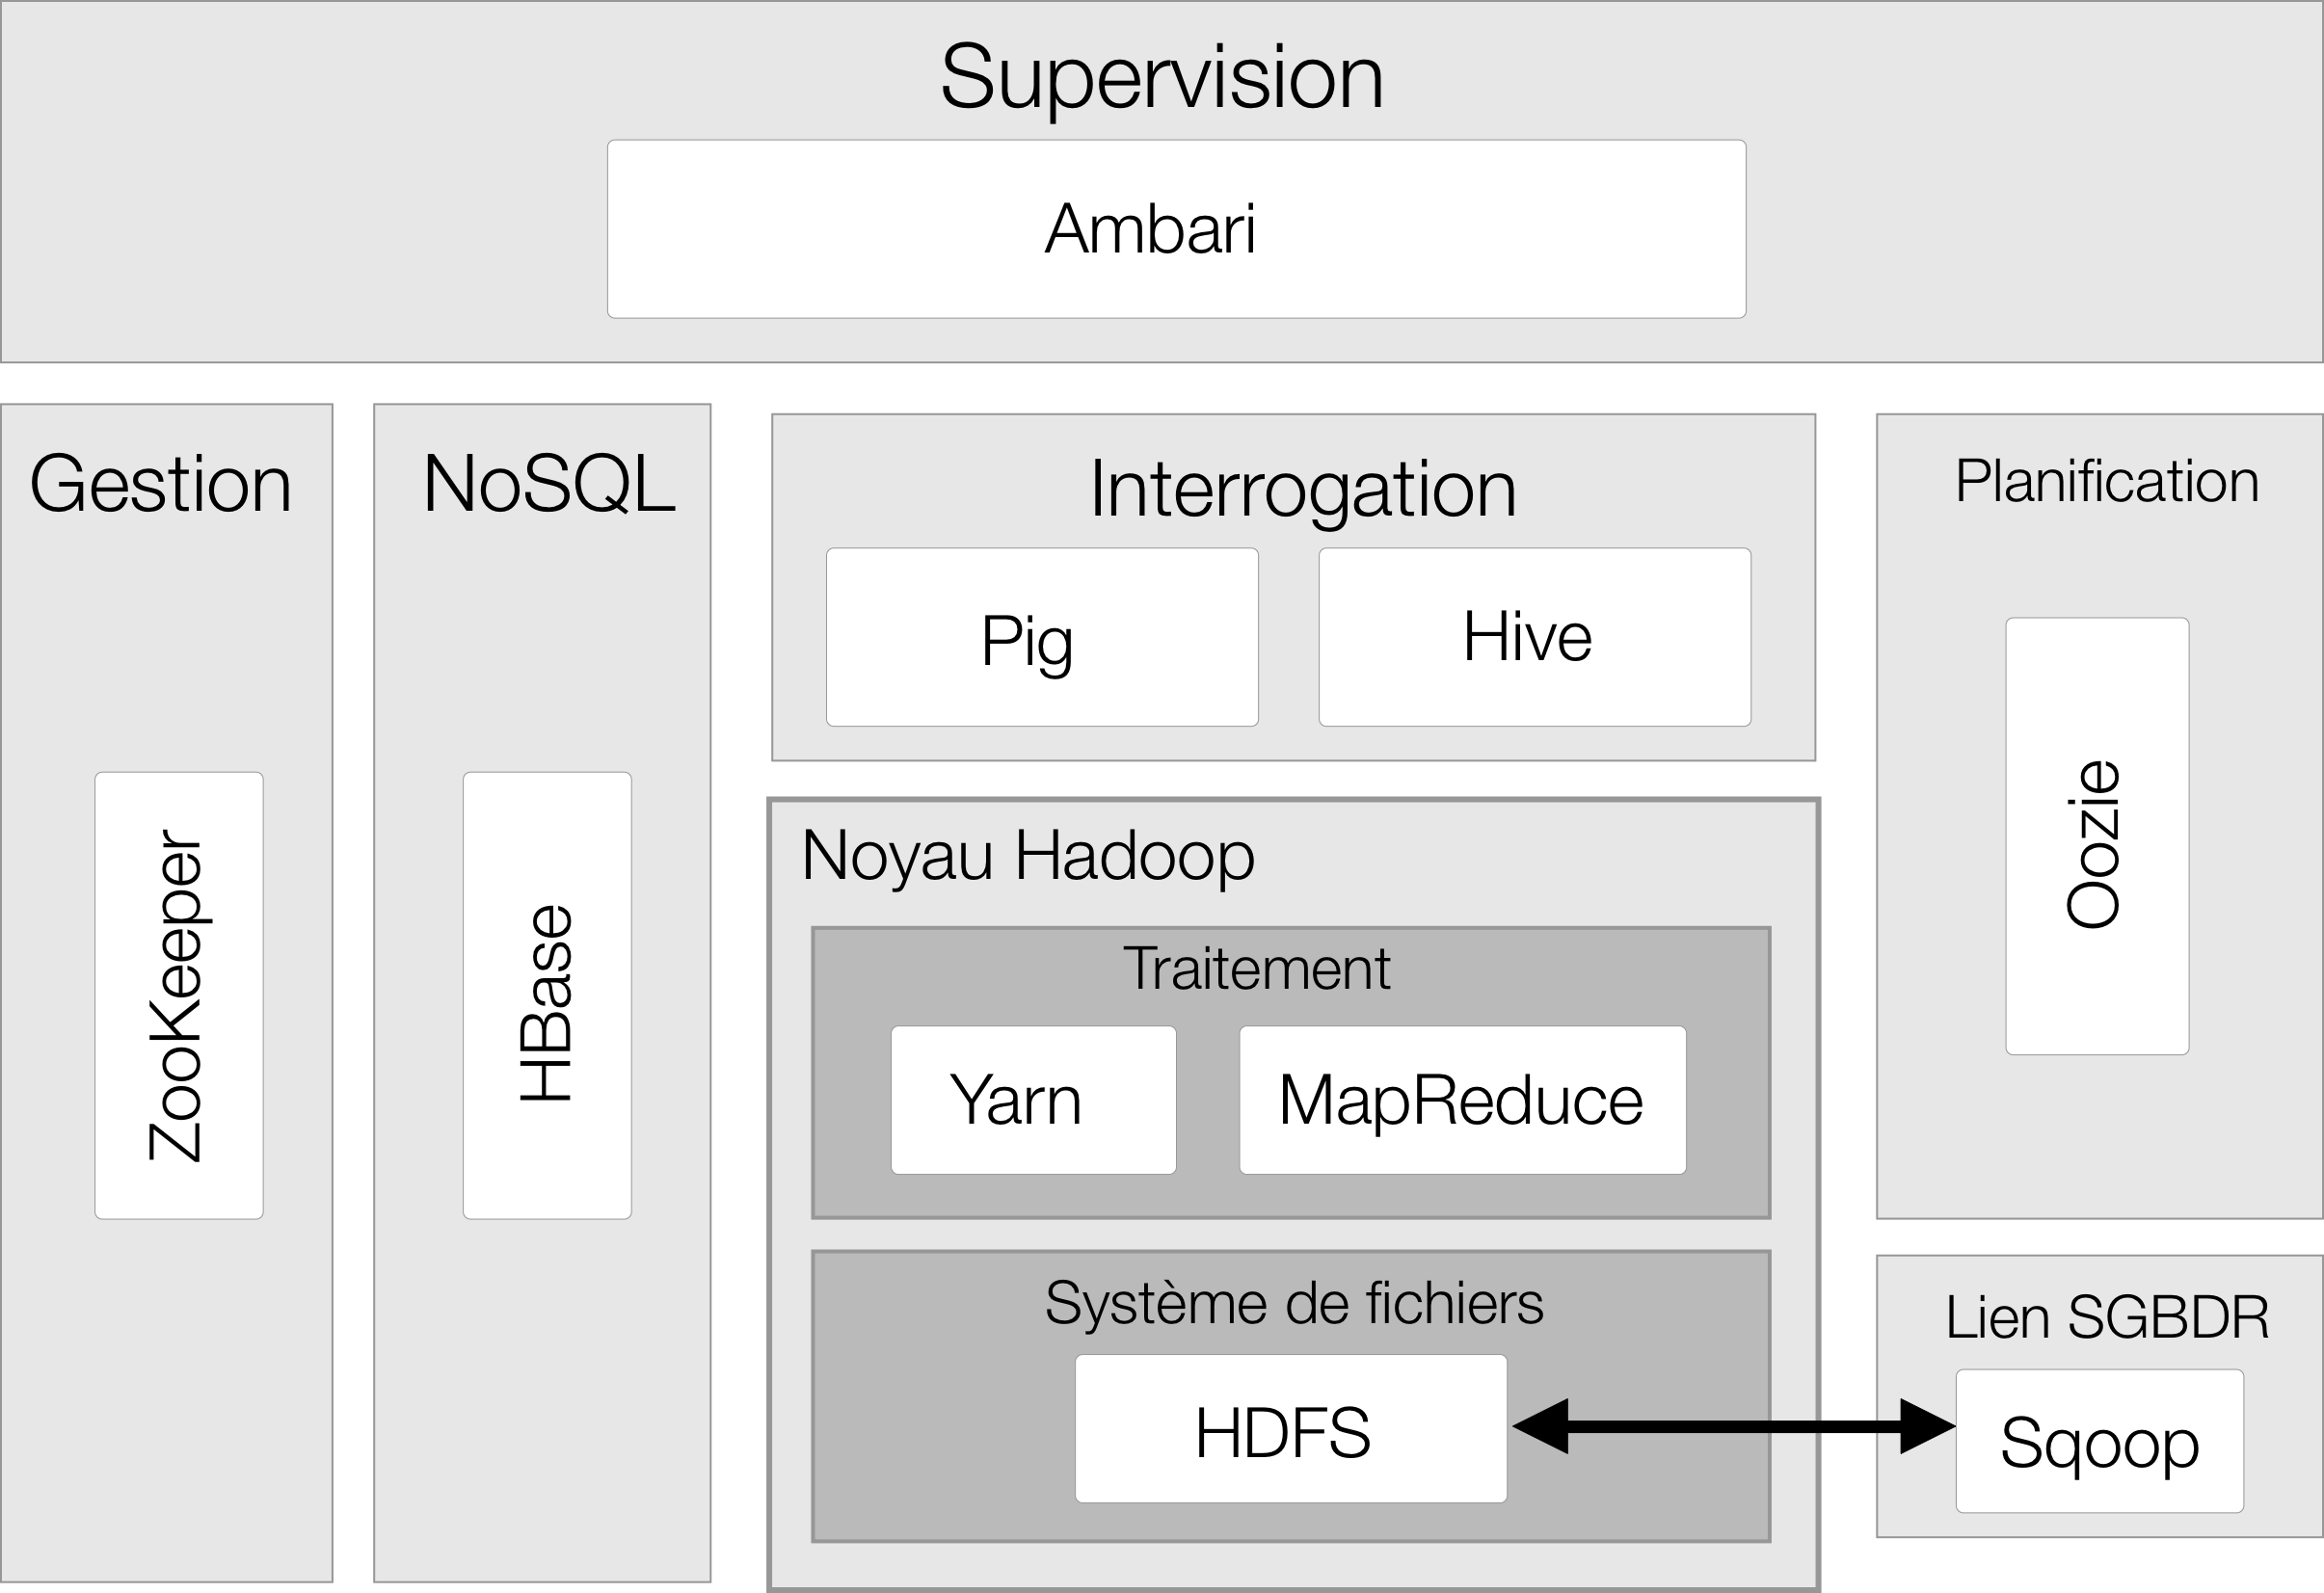
\includegraphics[width=0.9\textwidth]{hadoop_org}
\caption{Les différents composants des projets Apache autour de Hadoop}
\end{figure}
\paragraph{Hadoop Distributed File System}
Hadoop intègre un système de fichiers distribués qui prend en charge toutes les fonctions de réplication de données et de tolérance aux pannes sur un cluster. Ce système s'appelle HDFS qui signifie \textit{Hadoop Distributed File System}.
\par
HDFS a été conçu pour héberger des fichiers de très grande taille auxquels on accède le plus souvent en lecture seule. Comme tout système de fichiers, HDFS définit une notion de bloc qui correspond à la plus petite quantité de données qu'il est possible de lire ou d'écrire sur le disque. Cette taille est cependant beaucoup plus grande (environ 64 Mo) que dans les systèmes de fichiers ordinaires (512 octets), ceci pour optimiser les temps de transfert pour des fichiers volumineux.\par
L'architecture de base de HDFS est celle d'un système maître-esclave. Au sein d'un cluster HDFS, il existe un nœud maître, appelé NameNode, qui gère l'espace de nommage et qui associe les blocs aux différentes machines du cluster. Il gère toutes les métadonnées du système de fichier. Il existe des processus appelés DataNode, associés à chaque nœud, gère quant à eux les opérations de stockage locales. Sur instruction du NameNode, les DataNode procèdent aux opérations créations, de suppression ou de réplication des blocs.
\begin{figure}[H]
\centering
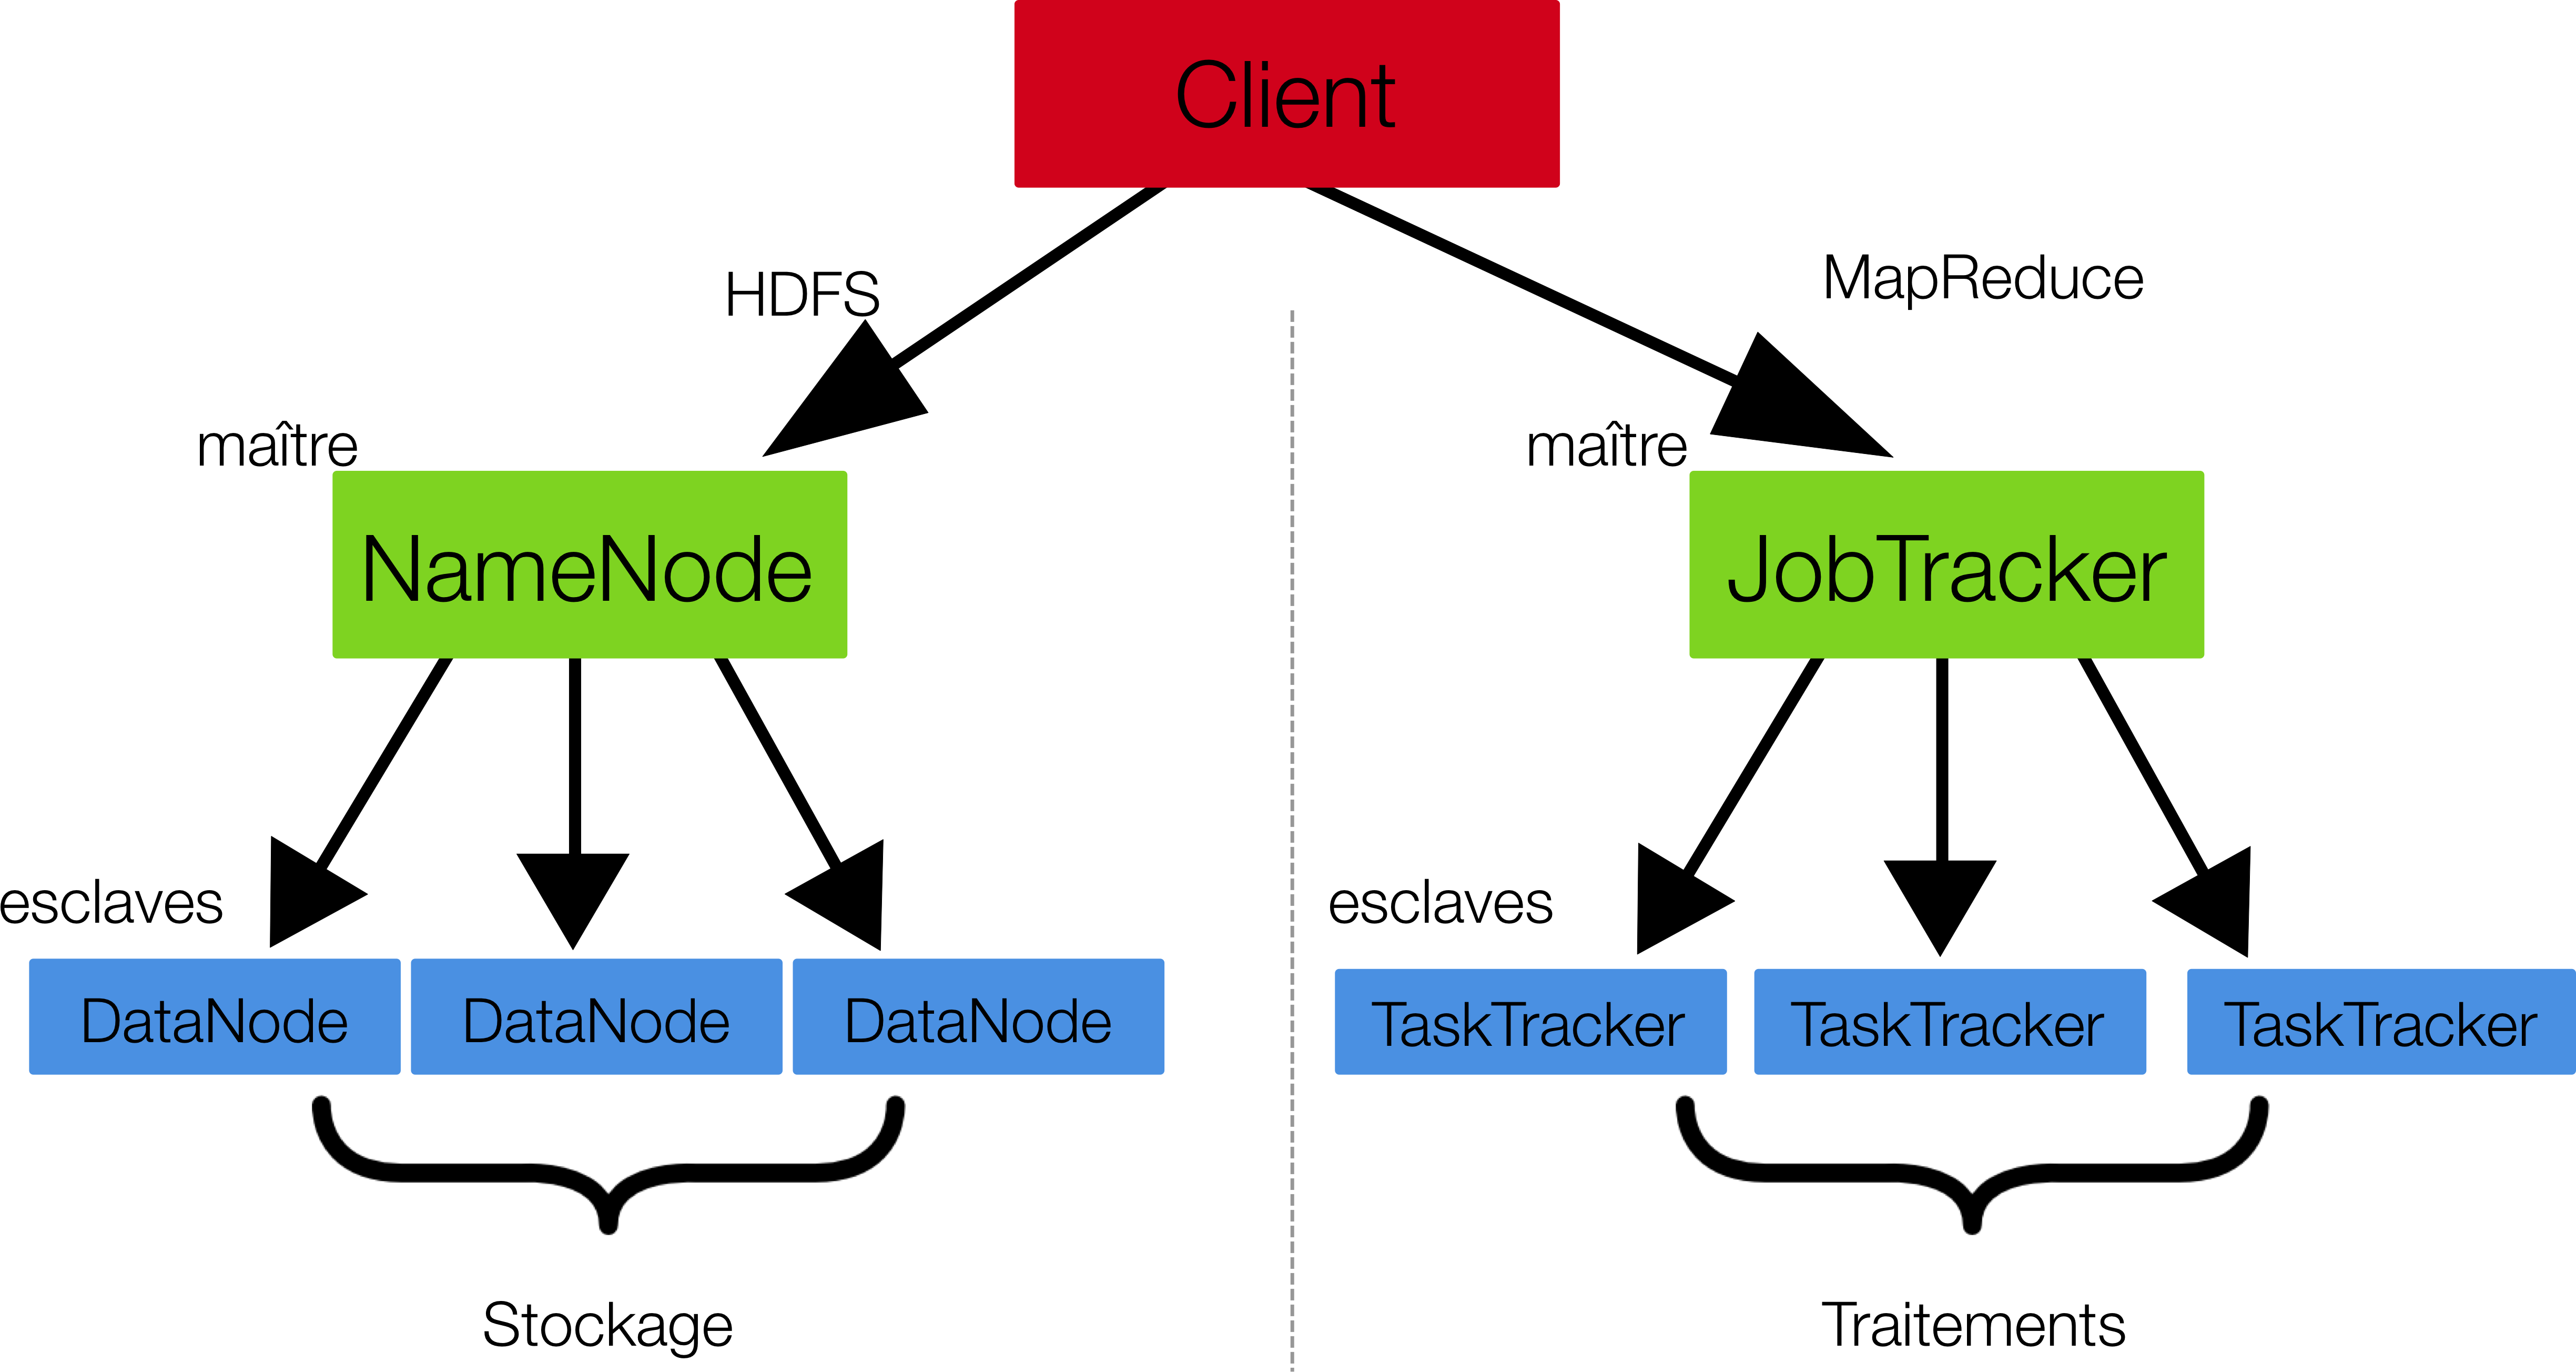
\includegraphics[width=0.9\textwidth]{hdfs}
\caption{L'articulation des \textit{NameNode} et des \textit{DataNode} au sein d'un cluster Hadoop}
\end{figure}
\paragraph{ZooKeeper}
L'objectif de ZooKeeper est de fournir un service de coordination de processus distribués au moyen d'un espace de nommage partagé hautement disponible en lecture. Un haut niveau de performance est assuré par une disponibilité des données en mémoire. Il peut être utilisé dans de nombreux contextes comme :
\begin{itemize}
\item l'utilisation d'un service de nommage,
\item la mise en place d'un système de configuration distribué,
\item l'utilisation d'un mécanisme de synchronisation distribué,
\item l'utilisation d'un système de file de messages,
\item la mise en place d'un système de notifications.
\end{itemize}
Le fonctionnement de ZooKeeper est similaire à celui d'un système de fichiers. Des registres de données de tailles limitées (moins d'un mégaoctet) appelées \textbf{znodes} sont identifiés au moyen d'un chemin. Ce qui le différencie à un système de fichiers ordinaire, c'est le fait de pouvoir associer des données à chacun des nœuds, somme si un fichier pouvait aussi être un répertoire et inversement. ZooKeeper a été conçu comme un outil de coordination qui permet de partager des données de configuration, de statut, de session, etc.
Zookeeper permet à une application de définir des notifications spécifiques à certains \textit{znodes}, appelés des \og watches \fg. Aussitôt que le contenu du nœud en question change, le client en sera notifié et le watch associé sera supprimé.
\par
Pour conclure, ZooKeeper est un framework Java qui contient des briques logicielles conçues pour développer des services de synchronisation et de coordination distribués, robustes et performants.
\paragraph{Pig}
Le développement d'une succession d'opérations \textit{map} et \textit{reduce} est une tâche complexe et délicate qui demande un haut niveau d'expertise en programmation et en conception. Augmenter le niveau d'abstraction utilisé pour décrire le processus de traitement est en l'occurrence la solution la plus naturelle. C'est la voie qu'emprunte Pig. Ce système comprend d'une part un langage de script, nommé Pig Latin, qui permet de définir un flot de transformations de données. De plus, Pig comprend aussi l'environnement d'exécution de ces scripts. Ceux-ci seront automatiquement compilés en une succession de jobs MapReduce, dispensant ainsi le développeur d'avoir à acquérir l'expertise en programmation MapReduce.
\paragraph{Hive}
\textit{Hive} est une infrastructure de datawarehouse construite sur Hadoop en vue de simplifier l'analyse d'ensembles de données très volumineux. Hive a été conçu à l'origine par les ingénieurs chez Facebook qui ne disposait pas  suffisamment de développeurs spécialisés dans la conception d'algorithmes MapReduce. L'objectif était alors de créer un système de traitement de données dont le langage de script serait aussi proche que possible du langage SQL ordinaire. Il ne restera plus qu'au système Hive de les compiler en jobs MapReduce. La plateforme d'exécution Hive et le langage HiveQL sont le résultat de ces travaux. C'est désormais un projet Apache qui bénéficie de contributions d'autres sociétés comme Netflix.
\paragraph{Oozie}
Apache \textit{Oozie} est un outil de planification de jobs Hadoop. Il permet de combiner plusieurs types d'opérations : MapReduce, Pig, Hive ou Sqoop en une seule unité logique. C'est donc essentiellement un outil conçu pour construire des combinaisons complexes et reproductibles d'opérations de transformations.
\paragraph{Flume}
Apache \textit{Flume} est une solution qui permet d'associer en temps réel différents flux de logs des serveurs web. Les données sont alors écrites dans le système de fichier HDFS. L'un des rôles principaux de Flume est d'isoler les applications clientes des pics de charge durant lesquels la quantité de données reçues excède celle qui peut être écrite sur disque. La conception de Flume garantit qu'aucune donnée n'est jamais perdue. 
\paragraph{Sqoop}
Apache \textit{Sqoop} est un outil qui permet de transférer efficacement de grands volumes de données entre Hadoop et un SGBDR. Sqoop est compatible avec les principaux SGBDR comme MySQL, Oracle, IBM DB2 ou Microsoft SQL Server. 
\subsubsection{Les principales distributions Hadoop}
Nous allons maintenant vous présenter les distributions de Hadoop les plus utilisés. Elles sont utilisables dans n'importe quel contexte technique.
\paragraph{Clourdera}
\begin{figure}[H]
\centering

\includegraphics[width=0.9\textwidth]{clouderaLogo}
\end{figure}
Cloudera a été fondée par des experts Hadoop et Doug Cuttings, le concepteur de Hadoop a rejoint les équipes Cloudera en 2009. Cloudera vend aussi bien des licences que du support et des formations. Cloudera propose par ailleurs une version open source de sa plateforme.
\par
Au noyau Hadoop d’ Apache, Cloudera ajoute ses propres interfaces graphiques d'administration, de gestion et de suivi, des outils de déploiement, des outils de gestion de la sécurité ainsi que des solutions d’intégration à un large éventail de produits. La suite est entièrement testée et documentée par Cloudera.
\par
À ce jour, c'est la distribution de Hadoop qui a le plus de déploiement référencé.
\begin{figure}[H]
\centering

\includegraphics[width=0.9\textwidth]{cloudera}
\caption{La plateforme Hadoop de Cloudera}
\end{figure}

\paragraph{Hortronworks}
\begin{figure}[H]
\centering
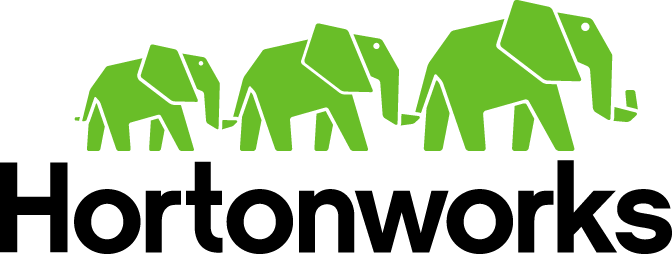
\includegraphics[width=0.9\textwidth]{hortonworks}
\end{figure}
Hortonworks a été fondée en 2011 par des spécialistes de Hadoop chez Yahoo. C'est une des seules à utiliser 100\% des composants open source Apache sans n'y rajouter aucune modification. L'objectif de Hortonworks est de faciliter l'adoption de la plateforme Hadoop d'Apache. Hortonworks est aussi un grand contributeur au noyau de la plateforme Hadoop. Le modèle économique de Hortonworks consiste essentiellement à vendre du support et des formations.
\begin{figure}[H]
\centering
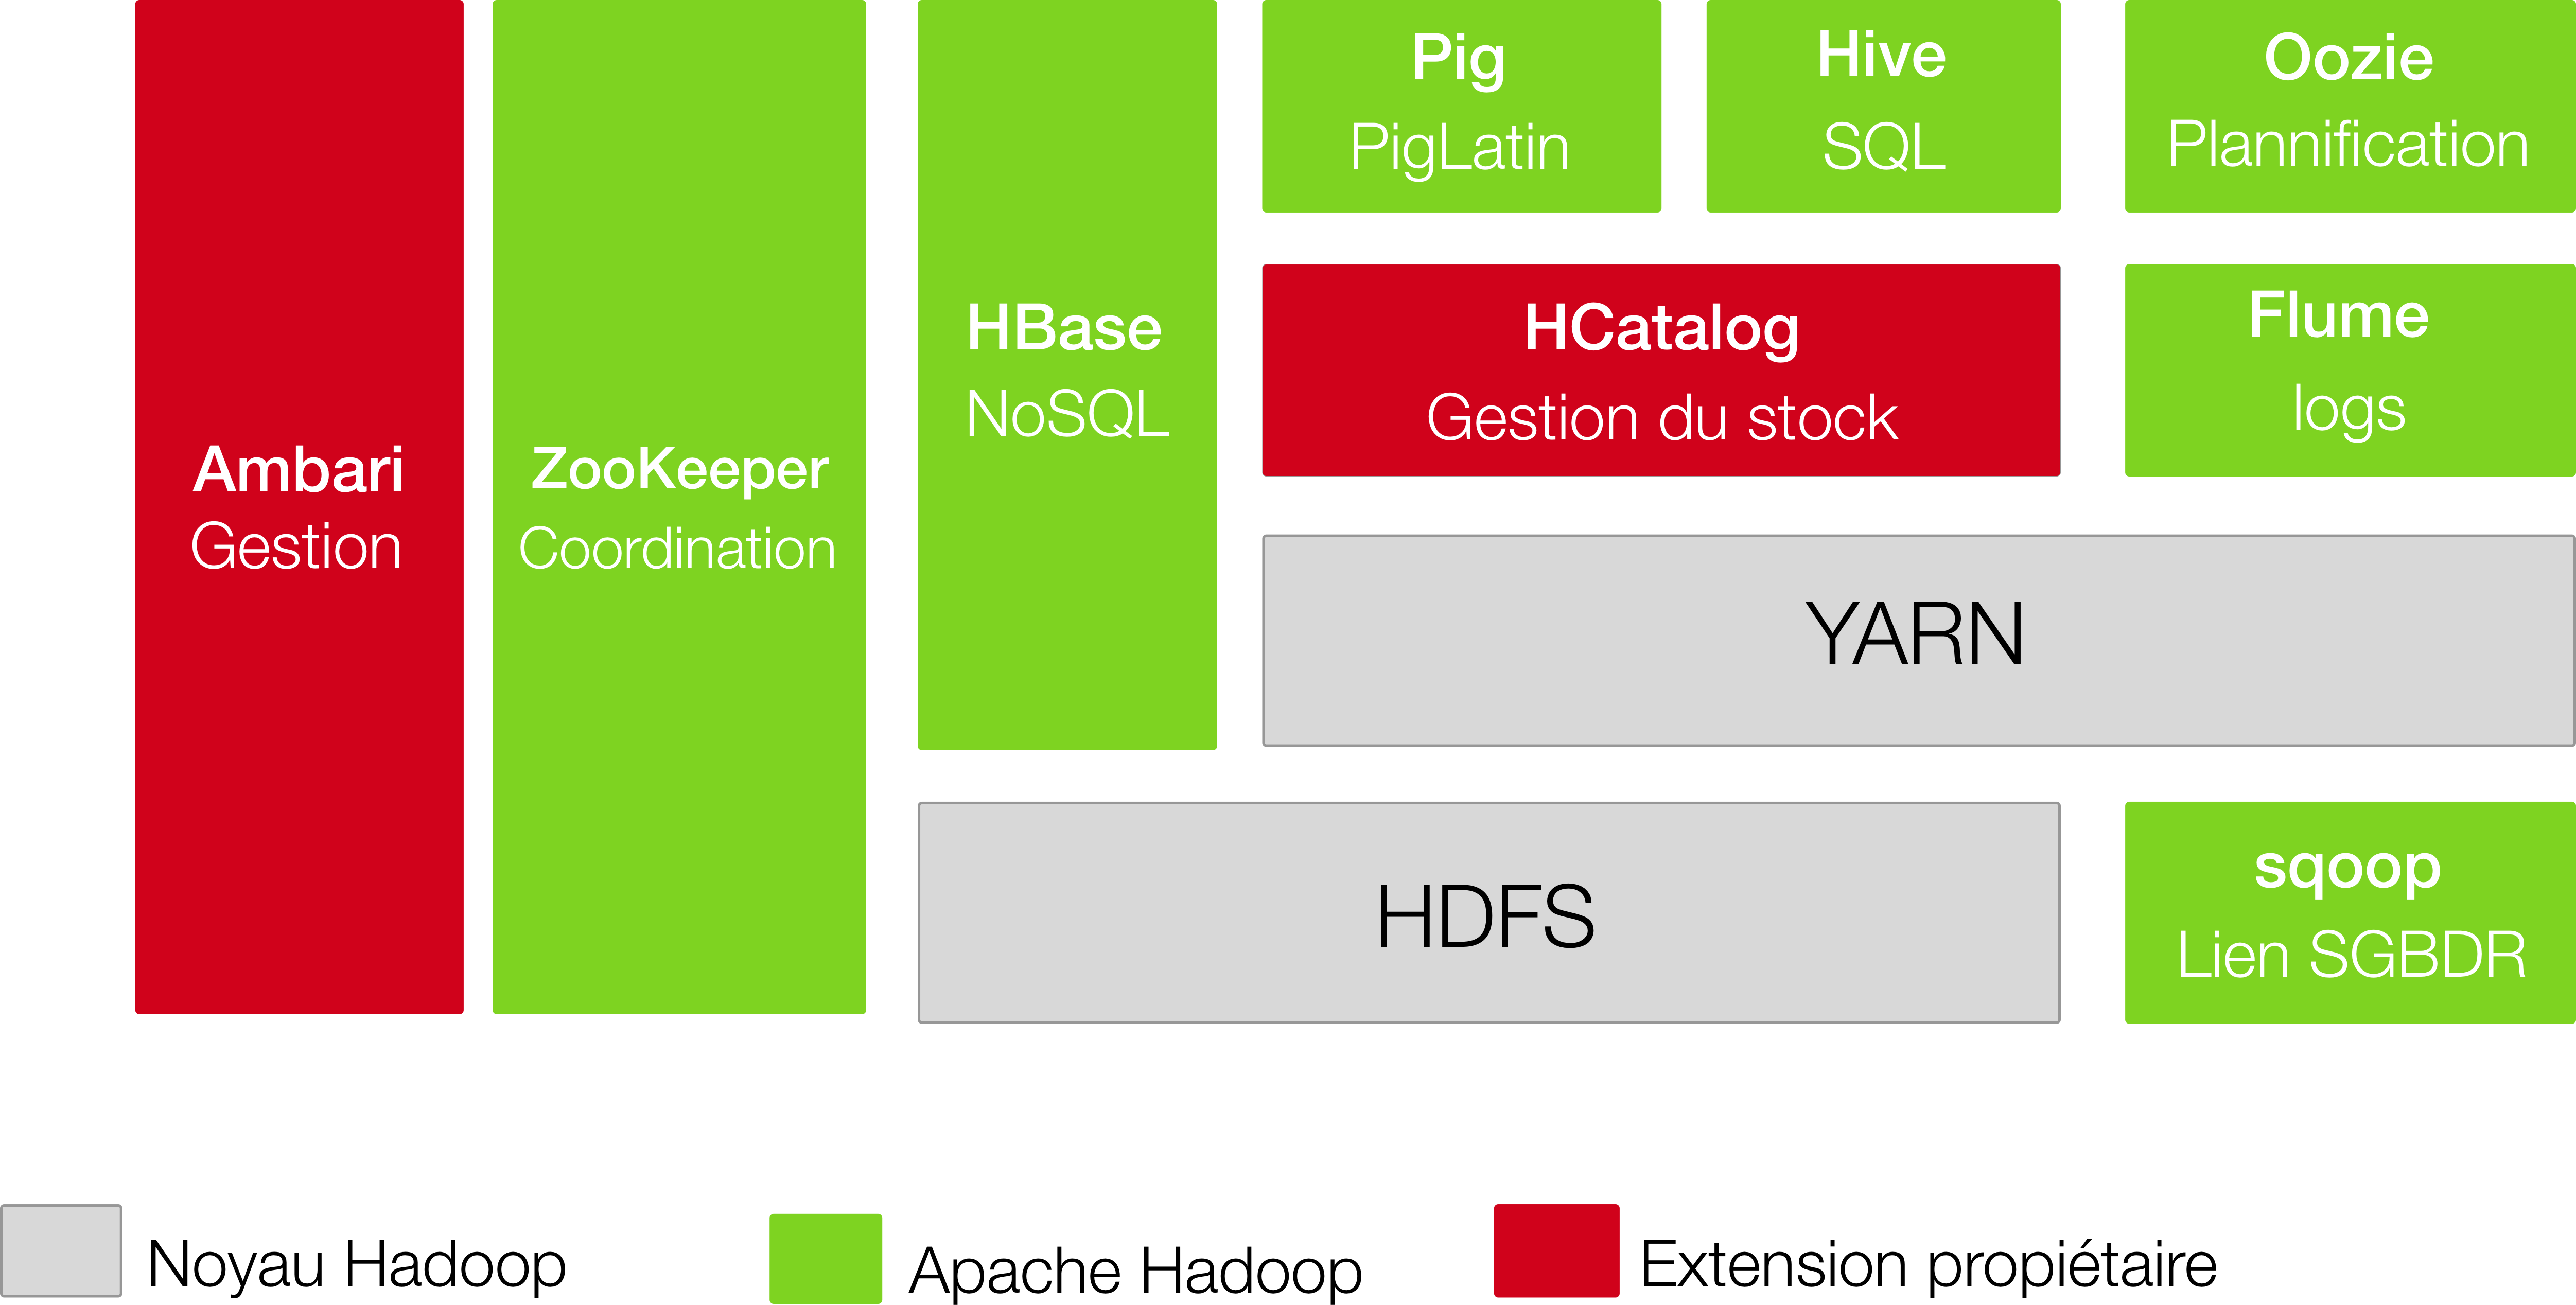
\includegraphics[width=0.9\textwidth]{Horton}
\caption{La plateforme Hadoop de HortonWorks}
\end{figure}
\paragraph{MapR}
\begin{figure}[H]
\centering

\includegraphics[width=0.9\textwidth]{MapR}
\end{figure}
MapR est une société californienne, fondée en 2009 par des collaborateurs de Google. Elle propose une distribution de Hadoop qui se veut particulièrement facile d'utilisation. Elle enrichit le noyau Hadoop de solutions propriétaires et propose trois distributions : M3 qui est gratuite, M5 qui ajoute des fonctionnalités de haute disponibilité et M7 enfin qui intègre une base de données haute disponibilité qui ré implémente TAPI de HBase. Elle utilise un système de fichiers propriétaires, MapR FS au lieu du système HDFS d’ Apache pour accroître les performances et propose également sa propre implémentation de MapReduce : MapR MapReduce.
\begin{figure}[H]
\centering
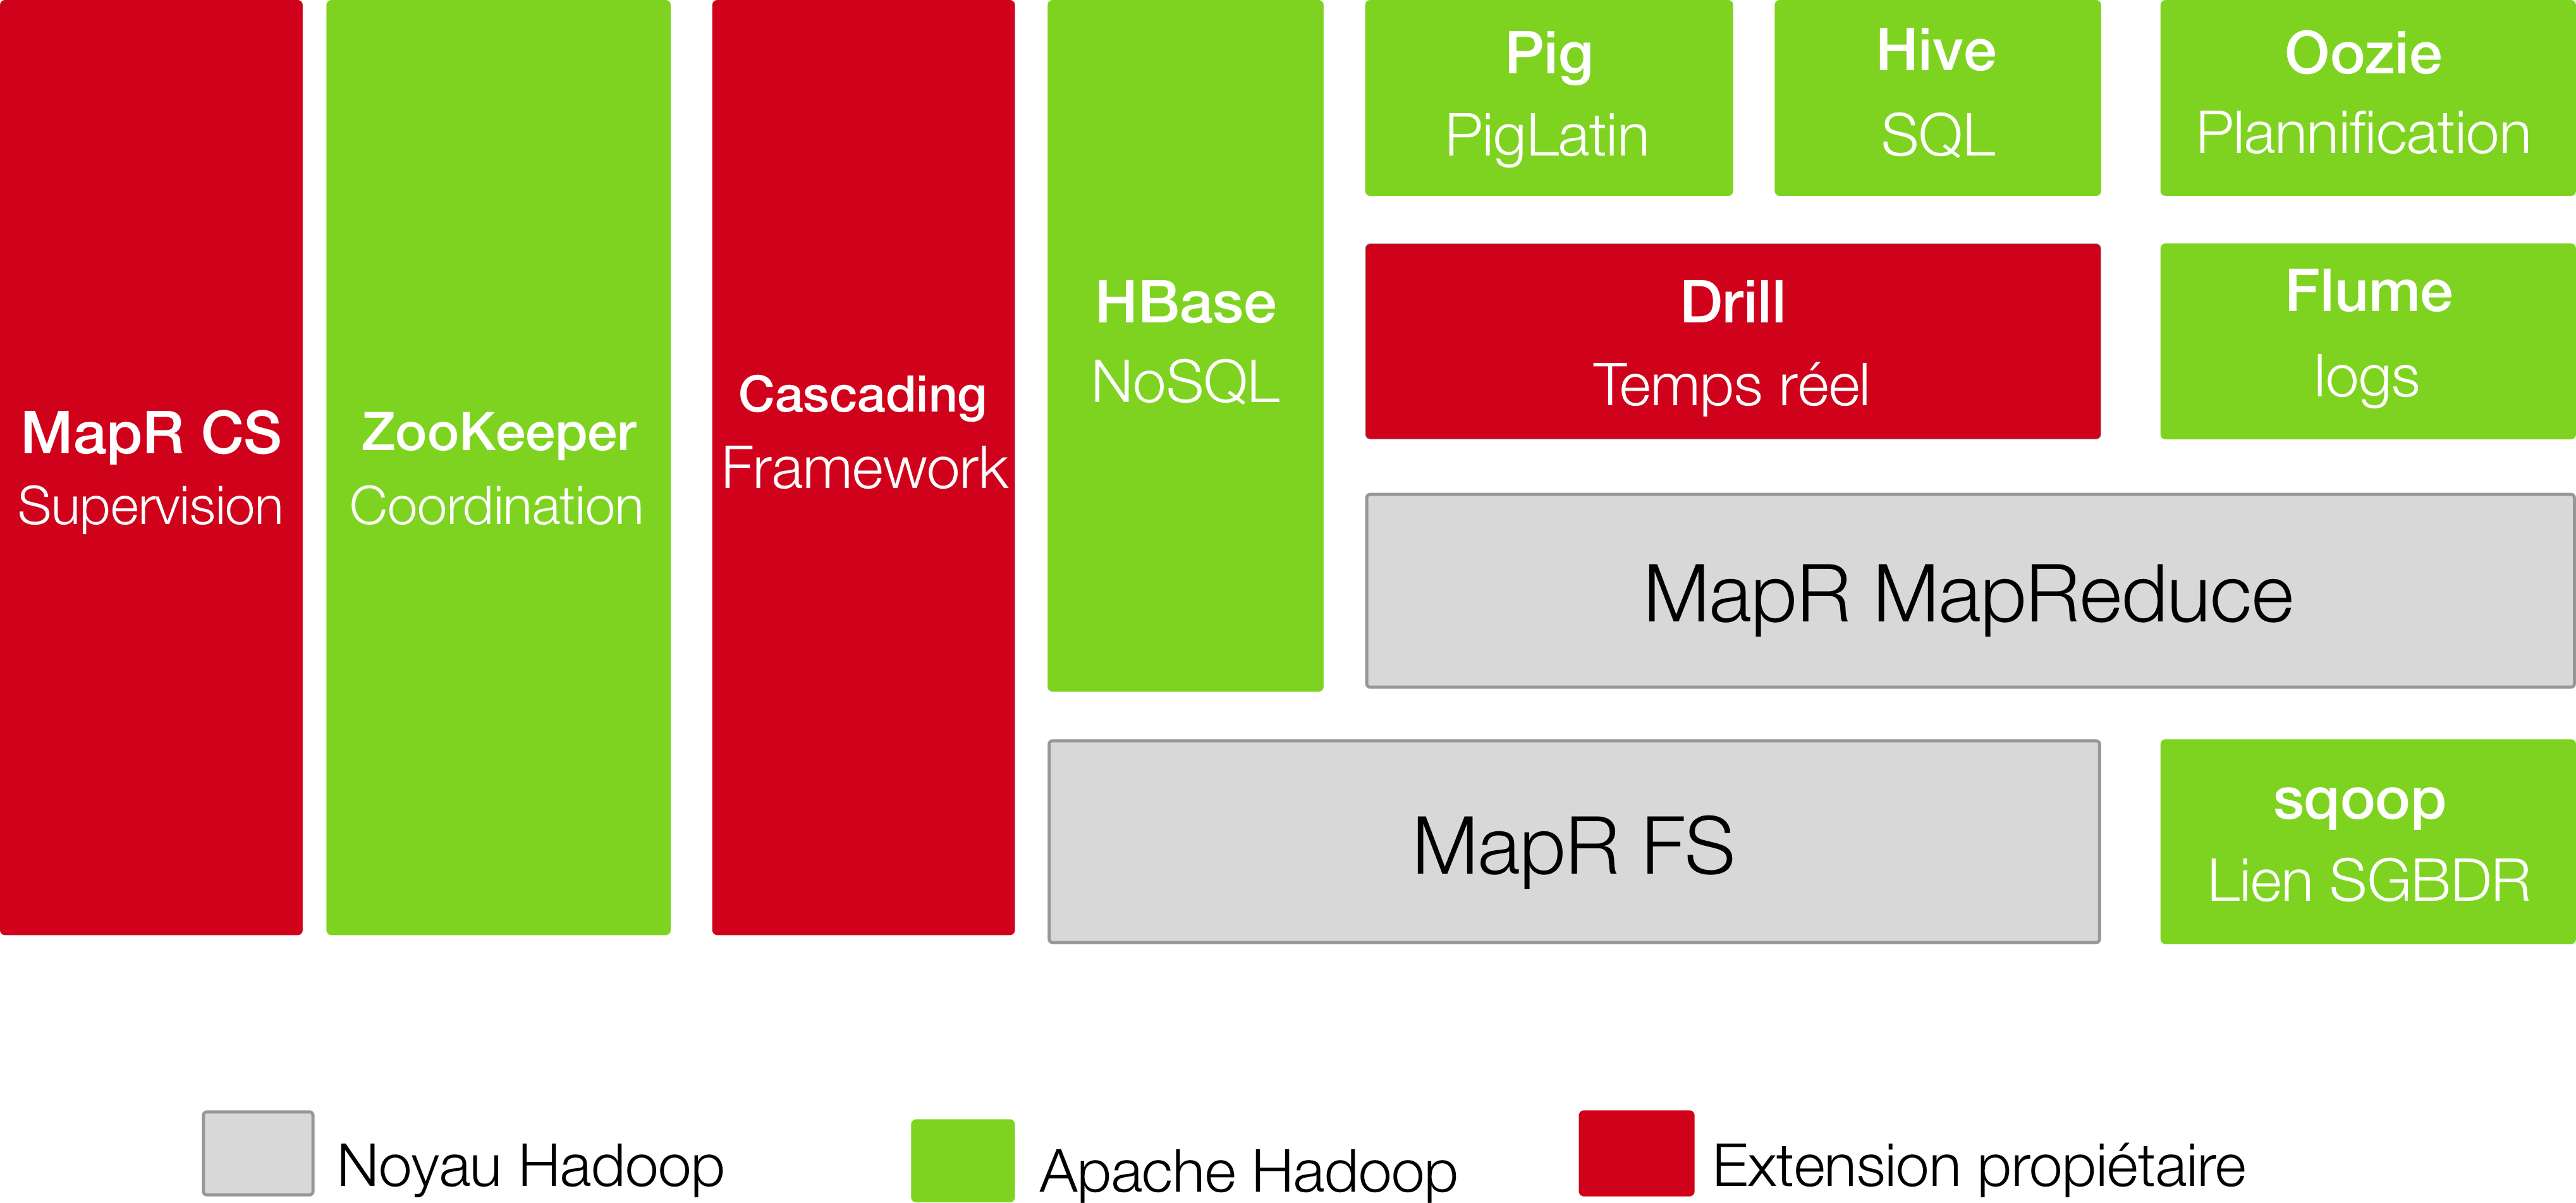
\includegraphics[width=0.9\textwidth]{Mp}
\caption{La plateforme Hadoop de MapR}
\end{figure}
\paragraph{Amazon Elastic MapReduce}
IMAGE Amazon Elastic MapReduce \\
\textit{Elastic MapReduce} (EMR) est une solution Hadoop dans le cloud proposée par Amazon depuis 2009. EMR est une solution idéale dans les situations où l'on cherche à disposer ponctuellement d'une importante puissance de traitement et de stockage. La solution permet d'économiser aussi bien les coûts liés à l'acquisition des compétences nécessaires au déploiement de Hadoop que l'achat des serveurs. Au prix toutefois d'une limitation des fonctionnalités puisque parmi les composants Hadoop seuls Pig et Hive sont inclus dans le package EMR. On aura tout intérêt par ailleurs à effectuer un rapide calcul du coût du transfert et d'hébergement des données si l'on veut éviter de mauvaises surprises.
 
EMR peut être utilisé avec une large panoplie d'outils tiers, qu'il s'agisse de l'environnement de développement, du transfert des données, de la visualisation ou de la BI. Enfin, notons qu'il est également possible d'utiliser la distribution MapR sur EMR.
\subsection{Outils mathématiques}
On le sait, les mathématiques font partie intégrale du Big Data et lui sont indispensable. La vague de données que le Big Data a apportées a contraint les mathématiques à s'adapter à un tel volume données. Pour le Big Data, les mathématiques seront utilisées dans un premier temps dans un processus d'analyse de données, ensuite il va falloir les explorer et enfin les traduire.
\subsubsection{Data mining}
Le Data Mining est en fait un terme générique englobant toute une famille d'outils facilitant l'exploration et l'analyse des données contenues au sein d'une base décisionnelle. Les techniques mises en action lors de l'utilisation de cet instrument d'analyse et de prospection sont particulièrement efficaces pour extraire des informations significatives depuis de grandes quantités de données.\par
Au contraire des méthodes classiques d'analyses statistiques, cet instrument d'analyse est particulièrement adapté au traitement de grands volumes de données. Avec l'augmentation de la capacité de stockage des supports informatiques, un maximum de renseignements seront captés, ordonnés et rangés au sein du Data Warehouse. Avec le Data Mining, ces gigantesques bases de données sont exploitables.
\par
Différentes techniques sont proposées. Elles sont à choisir en fonction de la nature des données et du type d'étude que l'on souhaite entreprendre.\par

Pour commencer l'analyse de données il faut tout d'abord les collecter, c'est une phase absolument essentielle et la plus importante. On n'analyse que des données utilisables, c'est à dire "propres". On n'hésitera pas à extraire de l'analyse les données de qualité douteuse. Bien souvent, les données méritent d'être retravaillées. Il faut s'assurer au final que la quantité de données soit suffisante pour éviter de fausser les résultats. Cette phase de collecte nécessite le plus grand soin. Ensuite, on analyse ces données récoltées à l'aide de méthodes que l'on expliquera plus tard. Et enfin, on étudie ces résultats afin d'en tirer de la valeur.
\subsubsection{Statistiques}
Les trois propriétés du Big Data, à savoir : Volume, Vitesse et Variété ont considérablement modifié l'approche statistique traditionnelle. En effet, en statistique traditionnelle plus un sondeur va acquérir de données plus le pourcentage d'erreur sera faible. Dans le cadre du Big Data c'est l'inverse, on a beaucoup plus de données pour un seul individu. Pire, le nombre de variables peut même dépasser la taille même de l'échantillon en question. On appelle cela le Fléau de la Dimensionnalité.
\subsubsection{Apprentissage}
En 2000, le mathématicien David Donoho a dit « L'espace considéré apparaît immense, et les choses intéressantes sont rares. Tout ce qui est a priori possible ne se réalise pas nécessairement ». En effet, il fallait trouver des méthodes mathématiques permettant dans ces vastes espaces de classer des éléments, de regrouper des parties semblables de l'échantillon, d'identifier des traits récurrents ou invariants, de repérer des motifs, prédire quels facteurs expliquent tel effet, etc.\par
Souvent ces objectifs reviennent à tenter de prédire un comportement à partir de différentes variables. Cela revient à tracer la meilleure courbe passant par tout ces paramètres et à répéter ce processus sur un autre individu, c'est ce qu'on appelle : l'Apprentissage. Cependant plus il y a de variables (ou points), plus le risque que la courbe se complique et devienne vite impossible à calculer est grand.
\subsubsection{Machine Learning}
Le Machine Learning (Apprentissage automatique ou statistique en français) concerne la conception, l'analyse, le développement et l'implémentation de méthodes permettant à une machine de remplir des tâches difficiles ou impossibles à remplir par des moyens algorithmiques plus classiques. L'analyse peut concerner des graphes, arbres, ou courbes au même titre que de simples grandeurs scalaires.
\par
Les algorithmes utilisés permettent, dans une certaine mesure, à un système piloté par ordinateur, ou assisté par ordinateur, d'adapter ses analyses et ses comportements en réponse, en se fondant sur l'analyse de données empiriques provenant d'une base de données ou de capteurs.\\
La difficulté se trouve dans le fait que l'ensemble de tous les comportements possibles compte tenu de toutes les entrées possibles devient rapidement trop complexe à décrire dans les langages de programmation actuels. On confie donc à des programmes le soin d'ajuster un modèle permettant de simplifier cette complexité et de l'utiliser. Ce modèle est adaptatif, il prend en compte l'évolution de la base des informations pour lesquelles les comportements en question ont été validés, ce que l'on appelle « apprendre » ceci permet d'améliorer le système d'analyse ou de réponse, ce qui est une des formes que peut prendre l'intelligence artificielle.
\subsubsection{La visualisation des données}
La visualisation des données concerne aussi bien le data scientist que l’expert métier ou le décideur. Elle dévoile au premier ce que les statistiques ne révèlent pas. Elle fournit aux experts et aux décideurs le support de l’intuition et la contextualisation indispensable à une prise de décision.\par
En réalité la visualisation intervient à toutes les étapes du travail d’un data scientist :
\begin{itemize}
\item \textbf{Préparation des données} : Dans cette phase la visualisation pourra servir à détecter des valeurs aberrantes ou des valeurs manquantes.
\item  \textbf{Choix d'un modèle} : À ce stade, on pourra valider certaines hypothèses comme la linéarité de certaines relations par exemple.
\item \textbf{Apprentissage} : Un data scientist peut guider l'apprentissage en supprimant certaines variables peu prédictives ou en construisant de nouvelles variables plus prédictives. La visualisation pourra ainsi contribuer à identifier quels sont les couples de variables les plus corrélées.
\item  \textbf{Optimisation d'un modèle} : Ici, il s'agit par exemple de vérifier que le modèle n'a pas subi de surapprentissage. Des courbes qui montrent l'évolution parallèle des erreurs de prédictions sur les ensembles d'apprentissage et de tests en fonction des paramètres ajustables du modèle permettront de trouver les paramètres optimaux.
\item \textbf{Prédiction} : La visualisation permet de partager l'information tout en la rendant intelligible à des experts métiers sans connaissances statistiques particulières.

\end{itemize}
\section{Conclusion}
Le Big Data qui correspond à un très grand volume de données provenant de diverses sources représente un enjeu considérable dans notre société en développement. Que ce soit dans le domaine du  marketing, dans les télécommunications ou encore la surveillance, le Big Data a une valeur très importante dans pratiquement tous les domaines et concerne peu à peu tous les secteurs d'activités. C'est pour cela que les ingénieurs développent continuellement de nouveaux système de gestion de base de données afin d'optimiser la manipulation du Big Data. 

\newpage
\section*{Liens}
https://www-01.ibm.com/software/fr/data/bigdata/ \\
http://www.lebigdata.fr/definition-big-data \\
http://www.bigdataparis.com/guide/Guide\_du\_Big\_Data\_2013\_2014.pdf \\
http://mylittlebigweb.com/infographie-big-data/ \\
https://fr.wikipedia.org/wiki/Open\_Source\_Initiative \\
https://fr.wikipedia.org/wiki/R\%C3\%A9trolien \\
http://www.piloter.org/business-intelligence/datamining.htm \\
https://fr.wikipedia.org/wiki/Propri\%C3\%A9t\%C3\%A9s\_ACID \\
\textbf{Enjeux et usages du Big Data} - \textit{Christophe Brasseur} - 2013 \\
\textbf{Big Data et Machine Learning} - \textit{Pirmin Lemberger, Marc Batty, Médéric Morel, Jean-Luc Raffaëlli} - 2015


\end{document}
